
% this file is called up by thesis.tex
% content in this file will be fed into the main document
    \graphicspath{{Background_Folder/figures/PNG/}{Background_Folder/figures/PDF/}{Background_Folder/figures/}}

%: ———————-- introduction file header ———————--
\chapter{Background}
This chapter provides the necessary background information and technical details required to understand the main results of this thesis and their implications to related fields of physics. These include both the theoretical framework we will use and the real world phenomena to which it relates \colorbox{red}{ }. \textcolor{red}{As the title hints}, in this text, we will concern ourselves with the study of \textcolor{red}{$2+1$ dimensional} systems at finite density. We will approach the study of these two dimensional systems through the framework of \textit{\textcolor{red}{q}uantum \textcolor{red}{f}ield \textcolor{red}{t}heory} (QFT). 

    There are two important aspects of QFT that will play a major role for us. One of them is the relation between the grand canonical statistical partition function and QFT. The other aspect is the distinct way in which the gauge principle manifests itself in 2+1 dimensional theories. The latter is addressed in \textcolor{red}{S}ection (\ref{CS_sec}), where we review the basics of \textit{Chern-Simons theory}. The former is discussed in \textcolor{red}{Subs}ection (\ref{GCE_sec}), where we will spend time reminding ourselves of some basic statistical mechanics. 

   % After we have covered these, we will turn to the physics this formalism aims to address in \ref{phys_app_sec}. We will review the \textit{Landau-Ginzburg  paradigm} \ref{Landau-Ginzburg_sec} of symmetry breaking and phase transitions, its inability to account for all phases observable in nature and where topological phases of matter fit in this picture.

    After we have covered these, we will spend some time looking at the problems of the \textit{fractional and integer quantum hall effects} (FQHE/IQHE) in \textcolor{red}{S}ection (\ref{FQHE_sec}) and emphasize their relation to Chern-Simons matter theories. This will help us understand the applications and motivate the study of the models we are concerned with in this text.

    Then, we shall continue by reviewing the properties of \textit{vortices} in \textcolor{red}{S}ection (\ref{vortices_sec}). Specifically, we look at vortices in the abelian Higgs model, pure abelian Chern-Simons theory with scalar matter and the mixed case where both classical Maxwell dynamics and the topological Chern-Simons term play a role. We emphasize the importance of a \textit{Bogomol'nyi-Prasad-Sommerfield (BPS)} \cite{Bogomolny:1975de, Prasad:1975kr} bound for these systems. Finally, we discuss some subtleties relating to non-abelian vortices.

    We continue by addressing \textit{Fermi-Bose and particle-vortex dualities} in \textcolor{red}{Section} (\ref{Fermi-Bose_sec}), which were the primary motivation for this work. We provide the relevant information about CFTs and RG flows in order to keep the presentation self-contained. We outline important aspects of the dualities in order to highlight where our work fits in that context.

    Finally, we include a section concerning the physics of \textit{non-commutative} field theory and its relation to the theory of fluids. In particular, we include the description of the \textcolor{red}{q}uantum Hall fluid in terms of a \textit{'fuzzy'} underlying space, in which the coordinates do not commute. We shall see that this description is a Chern-Simons theory and it seems to arise naturally out of the ground state in the finite density non-abelian model that we have studied.

        \section{Chern-Simons Theory} \label{CS_sec}
    Chern-Simons (CS) theory is a very unusual type of QFT both in its origin and its applications. It is a testament to the power and universality of mathematics, first conceived of as an abstract tool in the theory of differential operators and their connections to topology \cite{Chern:1974ft}, it has grown to encompass many facets of modern physics and mathematics. From the computation of knot invariants \cite{Witten:1988hf} to the prediction of non-abelian anyons \cite{Moore:1991ks}, which are the ingredients necessary for performing a topological quantum computation \cite{RevModPhys.80.1083} -- currently one of the most promising approaches to fault tolerant quantum computation \cite{Kitaev:1997wr}, due to the topological stability of the qubits. \textcolor{red}{CS} theory is an example of a topological field theory (TQFT) of \textit{Schwarz type} \cite{Schwarz:2000ct}, which means that it is independent of the metric and so any observable is related to a topological invariant. \textcolor{red}{The Einstein-Hilbert action in 2+1 dimensions can be written as the CS action \cite{Achucarro:1987vz}. This means that studying CS theory also provides insight into} three dimensional gravity \cite{Carlip:2005zn, Deser:1982vy, Witten:2007kt}. \textcolor{red}{CS theory also} provides a field theoretic explanation for the \textcolor{red}{q}uantum Hall \textcolor{red}{e}ffect and anyonic physics \cite{Zee, Tong:2016kpv}, has been instrumental in the classification of rational 2D CFTs \cite{Moore:1989yh}, creates a bridge between theoretical physics and knot theory \cite{Witten:1988hf} and, recently, it has uncovered an equivalence between two types of matter, previously thought to have been fundamentally different -- namely \textit{Fermi-Bose duality} \cite{Aharony:2015mjs} \cite{Aharony:2012nh, Giombi:2011kc, Aharony:2011jz, Giveon:2008zn}. These are among the most noteworthy applications of CS theory. Therefore, in this section we justly take the time to review essential aspects of CS theory. Most of the results seen in this section can also be found in the excellent review by \textit{Dunne} \cite{Dunne:1998qy}.

    In the study of fundamental physics, we should assume that any term in the Lagrangian that is not forbidden by a basic principle (\textit{e.g.} a symmetry or gauge-invariance) should be included in order to account for all aspects of the system at hand. From gauge theory we are familiar with the idea of introducing a gauge field to render a Lagrangian gauge invariant and then includ\textcolor{red}{ing} a gauge-invariant Yang-Mills term that is responsible for the dynamics of the gauge potential. Modulo subtleties, this is true in any number of dimensions. Taking these subtleties into account, it turns out that in 2+1 dimensions, the Yang-Mills term is not the only gauge invariant term one can include. One can write down a term in the action, which is the integral of a three-form, depending solely on the gauge field $A_{\mu}$. This term, whilst not manifestly gauge invariant, leaves the partition function unchanged under gauge transformations. This three-form is the Chern-Simons Lagrangian, which we write down here

\begin{equation}
    {\mathcal{L}}_{CS}= \kappa \, \epsilon^{\mu\nu\rho} \  \mathrm{Tr} \left[ A_\mu\partial_\nu A_\rho +{2\over 3} A_\mu A_\nu A_\rho \right].
\label{cslag}
\end{equation}
 \textcolor{red}{Here the coupling constant\footnote{Why we are referring to it as a \textit{coupling constant} will become apparent when we look at the inclusion of matter in CS models} $\kappa$ is conventionally referred to as \textit{the Chern-Simons level}. This name hints at the discrete nature of this quantity and we shall shortly see that, under certain conditions, one can derive a quantization conditions for $\kappa$.} The gauge field $A_\mu$ takes values in a finite dimensional representation $\mathcal{R}$ of the (semi-simple) gauge Lie algebra ${\mathfrak{G}}$. The $Tr$ operation is the standard matrix trace for an $dim(\mathcal{R})\times dim(\mathcal{R})$ matrix.  In an abelian theory, the gauge fields
$A_\mu$ commute, and so the trilinear term in \eqref{cslag} vanishes due to the
antisymmetry of the $\epsilon^{\mu\nu\rho}$ tensor. In the \textcolor{red}{non-abelian} case (just as in Yang-Mills theory) we write
\begin{align}
    A_\mu=A_\mu^a T^a,
\end{align}
 where the $T^a$ are the generators of ${\mathfrak{G}}$ (for $a=1,\dots, dim({\mathfrak{G}})$), satisfying the commutation relations
 \begin{align}
    [T^a,T^b]=f^{abc}T^c,
 \end{align}
and the normalization 
\begin{align}
    \mathrm{Tr}(T^a T^b)=-\frac{1}{2}\delta^{ab}.
\end{align}

We can define the field strength tensor in the usual way for a non-abelian gauge theory
\begin{align}
    F_{\mu \nu} = \partial_{\mu}A_{\nu} - \partial_{\nu} A_{\mu} + [A_{\mu}, A_{\nu}].
\end{align}




    $F_{\mu \nu}$ transforms under a gauge transformation in such a way that any expression that is the trace of a string of F's is gauge invariant. \textcolor{red}{More precisely, under a gauge transformation $g\in G=exp\left[\mathfrak{G} \right]$, }
\begin{align}
    \textcolor{red}{F_{\mu \nu} \rightarrow F'_{\mu\nu} = g^{-1} F_{\mu \nu} g \implies \mathrm{Tr}\left[ F_{i_1 j_i} ...F_{i_n j_n} \right]= \mathrm{Tr} \left[F'_{i_1 j_i} ...F'_{i_n j_n} \right].}
\end{align}

    Since \textcolor{red}{the} Lagrangian \textcolor{red}{\eqref{cslag}} is written in terms of $A_{\mu}$ as opposed to $F_{\mu \nu}$, gauge invariance is not manifest.


    Before we delve into the details of the gauge invariance of this Lagrangian, it is helpful to venture into a quick digression about \textit{topology}. Topological invariants are such properties of spaces (and hence of field configurations defined on those spaces) that do not change under continuous transformations. And since most phenomena in the real world are continuous, we should expect that these invariants are important tools that we can use to better understand the physical world. Indeed, we shall see that these expectations are justified. 

    One way topologists use to classify spaces is through \textit{homotopy groups}. An example is the first homotopy group $\pi_1$ or the \textit{fundamental group}. This group is an indicator of the ``connectivity'' of a manifold. Its definition has to do with whether a given loop can be contracted to a point. More precisely, one can define a group at each point on a manifold, whose elements are equivalency classes of loops that start and end at that point \textit{and} are continuously deformable into each other. For example, if all loops on a given space can be contracted to a point, then the fundamental group $\pi_1$ is trivial, since all elements of the group are the identity. The group operation on these loops is such that we create a new loop from $g_1$ and $g_2$ by going around $g_1$ first, then followed by going around $g_2$. It turns out that loops that encircle a singular point (or hole in the space) $n$ times are \textbf{not} continuously deformable into loops that encircle said point $n'$ times, if $n \neq n'$. This is an intuitive way of understanding the fact that for each hole in the space-time manifold, the fundamental group acquires a \textcolor{red}{C}artesian factor of $\mathbb{Z}$. Meaning that loops can wind around singular points arbitrarily many integer number of times and the number of loops around one singular point is independent of the number around another such singular point.

    Such a classification is not restricted to loops but can also be applied to higher dimensional spheres. For example, the classes of mappings from the 3-sphere to 3-dimensional Euclidean space-time are classified by $\pi_3$. If $\pi_3$ is non-trivial, this tells us that not all gauge transformations are connected to the identity. Importantly, for the purposes of theoretical physics, we shall use the fact that $\pi_3\left(SU(N) \right)=\mathbb{Z}$ for $N\geq2$ is non-trivial \cite{Toda1959}. We shall now see how this fact plays a role in the gauge invariance of Chern-Simons.

    To convince ourselves of the gauge invariance, let us perform a gauge transformation
    \begin{align}
        A_{\mu} \rightarrow A'_{\mu} \equiv g^{-1} A_{\mu} g + g^{-1}\partial_{\mu} g, \qquad g\in \mathcal{G},
    \end{align}
    where $\mathcal{G}$ is a compact semi-simple Lie group.
    Under this transformation, the Lagrangian changes in the following way
    \begin{align}
        \mathcal{L}_{\text{CS}} &\rightarrow \mathcal{L}_{\text{CS}}  - \kappa \epsilon^{\mu \nu \rho} \partial_{\mu} \ \mathrm{Tr} \bigg[\partial_{\nu} g g^{-1} A_{\rho}  \bigg] - \frac{\kappa}{3} \epsilon^{\mu \nu \rho} \ \mathrm{Tr} \bigg[g^{-1} \partial_{\mu} g g^{-1} \partial_{\nu} g g^{-1} \partial_{\rho} g\bigg].
    \end{align}
    The first term is just a boundary term. \textcolor{red}{If we are either considering manifolds with no boundary or we insist that the gauge transformation approaches $0$ at $\infty$, this term vanishes.} \textcolor{red}{For an $SU(2)$ transformation, t}he second term turns out to be proportional to the \textit{winding \textcolor{red}{number} density} of the gauge transformation, whose integral is an integer $n$ homotopy invariant
    \begin{align}
        w(g) = \frac{1}{24 \pi^2} \epsilon^{\mu \nu \rho} \ \mathrm{Tr} \bigg[g^{-1}\partial_{\mu} g g^{-1} \partial_{\nu} g g^{-1} \partial_{\rho} g \bigg], \quad \int d^3x \ w(g(x)) = n \in \mathbb{Z}.
    \end{align}
    \textcolor{red}{The integral of $w(g)$ is also known as the \textit{Brouwer degree} of a mapping. Here, the factor of $24\pi^2$ is proportional to the volume of the SU(2) group and depends only on the choice of gauge group and the convention we have chosen for the trace of the product of two generators (the \textit{Killing form}). }

    \textcolor{red}{For the case of a mapping between one $n$-sphere and another $n$-sphere (which is indeed the case  for an $SU(2)$ gauge transformation on $S^3$), we are guaranteed that this quantity is a homotopy invariant by \textit{Hopf's theorem} \cite{Dugundji}. Hopf's theorem states that two mappings $f,g: S^n \rightarrow S^n$ are homotopic if and only if they have the same winding number.}

    \textcolor{red}{Another way of seeing that $w(g)$ is a homotopic invariant is by varying $g\rightarrow g+\delta g$ and showing that the integral of the first order variation of $w(g)$, which we define to be $\delta w(g)$, vanishes. Using the fact that $(g+\delta g)^{-1} = g^{-1} - g^{-1} \delta g g^{-1}$ to first order and the cyclicity of the trace, we can show that}
\begin{align}
    \textcolor{red}{   \int d^3x \, \delta w(g) = \frac{1}{24 \pi^2} \epsilon^{\mu \nu \rho} \int d^3 x \, 3 \partial_{\mu}\mathrm{Tr} \left[(g^{-1} \delta g) g^{-1} \partial_{\nu} g g^{-1} \partial_{\rho} g \right].}
\end{align}
\textcolor{red}{Using Stokes' theorem and requiring that the variation $\delta g$ vanishes at the boundary (or equivalently, considering a manifold without a boundary, which is the case for $S^n$), we see that}
\begin{align}
    \textcolor{red}{ \int d^3 x \, \delta w(g) =0.}
\end{align}
\textcolor{red}{Thus we see that the winding number is unaffected by small variations of the mapping.}

    Gauge transformations with a non-zero winding number are called \textit{large gauge transformations}. Another way of saying this, is that they are mappings that are \textit{not} continuously connected to the identity transformation. \textcolor{red}{Here we take a break from Chern-Simons theory to give a simple example to illustrate how these gauge transformations are different.}

    Suppose we have a complex scalar field $\varphi$ defined on  $S^1$
    \begin{align}
        \varphi: S^1 \rightarrow \mathbb{C},
    \end{align}
    such that $\varphi = f(\theta) e^{i \alpha(\theta)}$, where $f\in \mathbb{R}$ and $\theta$ describes the position on the $S^1$. Here the $e ^{i \alpha (\theta)}$ can be absorbed into a $U(1)$ gauge transformation. Below (Fig \ref{large_gauge}) we have represented pictorially the phase of the scalar at a point on the manifold (in this case $S^1$) as a red arrow pointing in a direction on the plane. In (a) we have $\alpha(\theta) = \frac{\pi}{2}$. It is not hard to convince ourselves that we can transform this configuration to $\alpha(\theta) =0$ by making the same infinitesimal changes at every point on $S^1$. Thus $\alpha(\theta) = \frac{\pi}{2}$ is an example of the familiar kind of ``small gauge transformation''. One can go from (a) to (b) by setting $\alpha =\theta - \pi$. However, in this case we see that there is no way to make small transformations that are continuous. Configurations (b) and (c) are said to be in a different homotopy class from (a), but they are in the same gauge equivalency class as (a).
    


\begin{figure}[htb]
	\centering
	\begin{tabular}{c@{\hspace{1.5cm}}c@{\hspace{1.5cm}}c}
		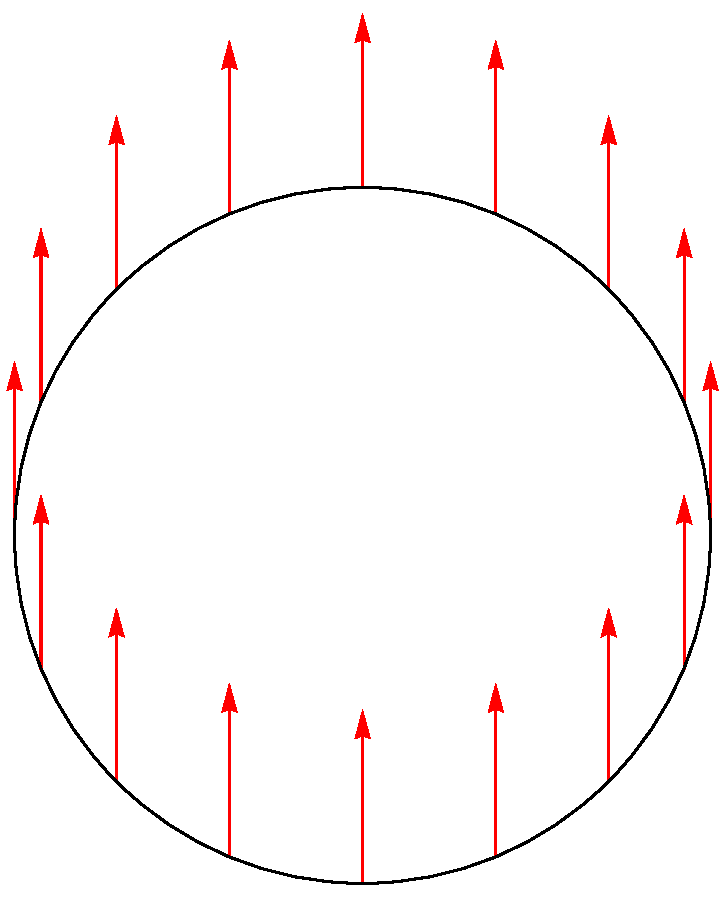
\includegraphics[scale=0.17]{lrg_gauge1.pdf} \text{(a)}  &  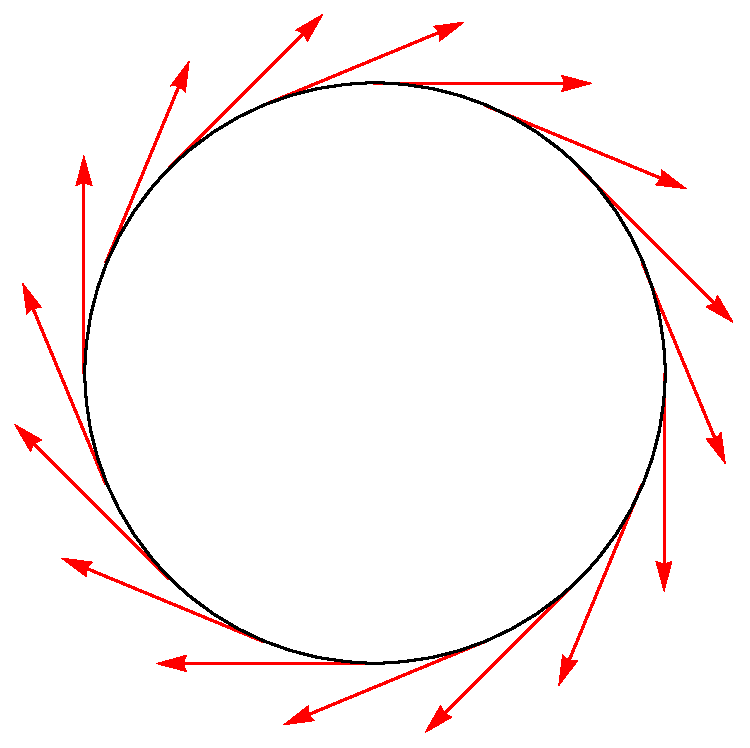
\includegraphics[scale=0.19]{lrg_gauge2.pdf} \text{(b)}  &
		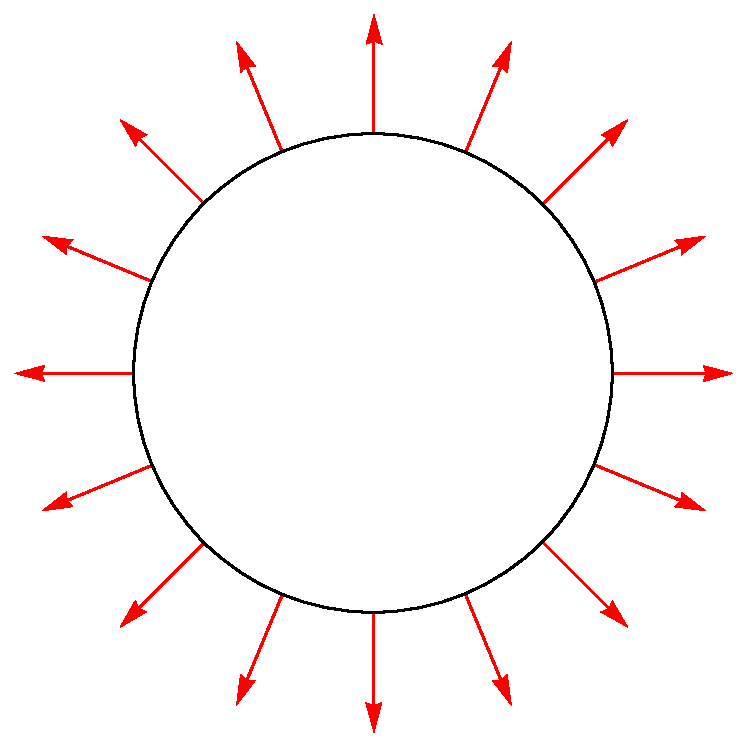
\includegraphics[scale=0.19]{lrg_gauge3.pdf} \text{(c)}
	\end{tabular}
    \caption[This figure provides a simple example that illustrates the idea behind a large gauge transformation.]{This figure provides a simple example that illustrates the idea behind a large gauge transformation. (a) is topologically distinct from the rest, yet they are all gauge equivalent configurations. } \label{large_gauge}
\end{figure}

As a final remark to counter the point that ``We don't live on a circle'', I shall say that when studying a non-singular circularly symmetric planar setup, we would require boundary conditions which identify the point at infinity with the same gauge-field configuration. It turns out that the point at infinity \textit{is} an $S^1$, so inevitably abelian gauge transformations \textit{would be} separated into distinct homotopy classes.

This above passage illustrates the essence of large gauge transformations in the simplest possible case, where we have a non-trivial homotopy group. The situation is precisely the same with more complicated homotopy groups but they just happen to be more difficult to visualize.

    Going back to the Lagrangian transformation law, we pick $g$, s.t. $\textcolor{red}{\int d^3 x} \,w(g)=n$. Therefore the action transforms as
    \begin{align}
        S_{\text{CS}} \rightarrow S_{\text{CS } }+ 8 \pi^2 \kappa n.
    \end{align}
    Here we see that the action is \textit{not} gauge invariant! However, keep in mind that what plays a role in the path integral is $e^{i S}$, which transforms as
    \begin{align}
        e^{i S_{CS}} \rightarrow e^{i 8 \pi^2 \kappa n} e^{i S_{\text{CS}}}.
    \end{align}
    This implies that if we set $\kappa = \frac{k}{4 \pi}$, where $k\in \mathbb{Z}$, we have restored gauge invariance, which means that we ought to include this term in the study of planar physics.

    \textcolor{red}{The previous discussion can be easily generali\textcolor{red}{s}ed to gauge groups other than $SU(2)$, which allow for non-trivial homotopies by simply adjusting the normalization of the winding number. The case of $SU(N)$ is identical, since one can consider an $SU(2) \cong S^3$ subgroup in $SU(N)$, which maps onto the space-time. Let us take the simplest example that differs from $SU(2)$, the case of $SO(3)\cong SU(2)/ \mathbb{Z}_2$. The normalization of $w_{SO(3)}(g)$ is half that of $SU(2)$, since $vol[SO(3)] = \frac{1}{2} vol[SU(2)]$. If $w_{SO(3)}(g)=n$, then the shift of the action becomes }
\begin{align}
    \textcolor{red}{S_{\text{CS}} \rightarrow S_{\text{CS}}+ 4\pi^2 \kappa n.}
\end{align}

\textcolor{red}{Setting $\kappa = \frac{k}{4 \pi}$ leads us to a quantization condition which requires an \textit{even} Chern-Simons level $k \in 2\mathbb{Z}$ in the case of an $SO(3)$ gauge group.}

\textcolor{red}{Next, we comment on the quantization of the Chern-Simons level in the case of a compact abelian gauge group. The same argument, where we compactify $\mathbb{R}^3 \rightarrow S^{3}$ and then perform gauge transformations with a non-trivial winding number, no longer applies for an abelian group, since $\pi_1(S^3)$ is trivial. In fact, the level for an abelian CS theory is not \textit{in general} quanti\textcolor{red}{s}ed \cite{Polychronakos:1990xq}. We can, however, derive a quantization condition with a small set of additional assumptions.}

\textcolor{red}{Those two assumptions are}
\textcolor{red}{
    \begin{itemize}
        \setlength\itemsep{1em}
        \item[$\circ$] Finite Temperature $T$.}\\
            \vspace{0.01em}
            \textcolor{red}{Studying a Quantum Field Theory at finite temperature is equivalent to Wick rotating into Euclidean space and compactifying the time direction to an $S^1$. This leads to a space-time of the form $S^1 \times M$, where $M$ is a 2-dimensional manifold.
        \item[$\circ$] Consistency of the theory in the presence of a magnetic monopole.}\\
            \vspace{0.01em}
            \textcolor{red}{As we have already touched upon in the Introduction, in 1931, \textit{Paul Dirac} considered the possibility of the existence of a magnetic monopole \cite{Dirac:1931kp}. This is contrary to the statement of Gauss's law for magnetism, which states that magnetic monopoles cannot exist (since for such a configuration we would have $\nabla \cdot B \neq 0$). Dirac's construction required the existence of a singularity associated with it. Later on, in 1975, \textit{Wu \& Yang} \cite{Wu:1975es, Wu:1976ge}  resolved the mystery of the Dirac string by showing how gauge fields are connected to the mathematical concept of \textit{fiber bundles}, thus showing that a proper definition of the vector potential of a monopole, should be defined in patches, which are related by gauge transformations on the intersections. Here we will consider the monopole on a sphere $S^2$. The presence of a monopole implies that
    \end{itemize}}
\begin{align}
    \textcolor{red}{\frac{1}{2\pi} \int_{S^2} F_{12} = 1.} \label{monopole_flux}
\end{align}
    \textcolor{red}{With this setup, we can now perform a large gauge transformation along the time manifold $S^1$, and study its effect on the Chern-Simons action. However, this would lead us to a result that is incorrect. The reason for this is that our definition of the Chern-Simons action is ambiguous for a non-trivial fiber bundle (read for a gauge field that is not globally defined). The correct way of approaching this problem is by defining the $U(1)$ Chern-Simons action as the boundary term of a 4-dimensional action \cite{Dijkgraaf:1989pz}}

\begin{align}
    \textcolor{red}{S=\frac{k}{4 \pi} \int_{B} F\wedge F,}
\end{align}
 \textcolor{red}{ Where $B$ is a four manifold that bounds $S^1 \times S^2$. Here we shall take $B= D\times S^2$, where $D$ is the disk with boundary $S^1$. We know that the size of the $S^1$ is $\beta= \frac{1}{T}$, as dictated by thermodynamics. This implies that the radius of the disk is $R_D=\frac{\beta}{2\pi}$. Since the total space-time is a direct product, we can write the field strength as a sum of contributions to the separate parts of the manifold} 
\begin{align}
    \textcolor{red}{F= F_D +F_{S^2}.}
\end{align}
 \textcolor{red}{Since the wedge product of 2-forms commute, we have }
\begin{align}
    \textcolor{red}{   S = \frac{k}{4\pi}\int_B F\wedge F = \frac{k}{2\pi} \int_B F_{D} \wedge F_{S^2}.}
\end{align}
\textcolor{red}{Let's consider a large gauge transformation on $S^1$. Let $A_D$ be the gauge field defined on the disk $D$ and let a position on that disk be described in polar coordinates $(r, \alpha)$, where $r$ is the radial position and $\alpha$ the polar angle. A candidate for a non-single valued function on the boundary of $D$ ($S^1$) is a transformation of the form }
\begin{align}
    \textcolor{red}{A_D \rightarrow A_D + \frac{r}{R_D} d\alpha. \label{non-gauge_gauge}}
\end{align}
\textcolor{red}{This is \textit{not} a gauge transformation on $D$, but it is a perfectly well-defined gauge transformation on $S^1$ and, as such, we expect the boundary theory to be invariant under it. Since (\ref{non-gauge_gauge}) is not a gauge transformation on $D$, $F_D$ changes}
\begin{align}
    \textcolor{red}{F_D \rightarrow F_D + d (r d\alpha) =F_D + dr \wedge d\alpha.}
\end{align}
 \textcolor{red}{This implies that the action changes accordingly }
\begin{align}
    \textcolor{red}{\delta S }& \textcolor{red}{= \frac{k}{2\pi} \int_B \frac{1}{R_D} dr \wedge d\alpha \wedge F_{S^2}}\\
    & \textcolor{red}{= \frac{k}{2\pi} \int_{S^1}  d\alpha \int_{S^2} F_{S^2}=2\pi k,}
\end{align}
 \textcolor{red}{where we have used Stokes' theorem, the monopole flux condition (\ref{monopole_flux}) and the fact that on the $S^1$, $r=R_D$. Just as in the non-abelian case, we see that if we would like the path integral over the boundary to remain invariant, we require that }
\begin{align}
    \textcolor{red}{\delta S \in 2\pi \mathbb{Z} \implies k\in \mathbb{Z}.}
\end{align}
\textcolor{red}{We remark that if the local definition of the Chern-Simons action had been used in this derivation, we would be off by a factor of 2, which would mean the level would be quanti\textcolor{red}{s}ed to only even integers, leading to incorrect physical predictions. Finally, it's important to note that even though the arguments above are classical in nature, there is a result that guarantees the non-renormalizability of the Chern-Simons level beyond 1-loop. This is known as the \textit{Coleman-Hill theorem} \cite{Coleman:1985zi, Khare:1994yv}  }
 \textcolor{red}{\subsubsection*{Equations of Motion}}
    Let us look at some physical properties that the action functional $S_{\text{CS}} = \int d^3x \, \mathcal{L}_{\text{CS}}$ possesses. Performing the functional variation, we get the equation of motion $F_{\mu \nu}=0$, implying only pure gauge solutions exist. This might make one wonder, what could possibly be so interesting about CS theory if the classical equations of motion are trivial!?
    The reason that this theory is in fact interesting and non-trivial, despite the fact that $F=0$, is two-fold. Firstly, CS is a topological field theory. It has trivial local properties. All of the physics is encoded in the topology of the manifold and in the non-local observables such as Wilson loops that require us to study the full quantum theory.

    The second way in which CS is interesting teaches us the old lesson that sometimes the whole is greater than the sum of its parts. In this case, adding matter or a Maxwell term to the Lagrangian alters the pure Maxwell/matter theories immensely. Let us see how these alterations play out.

    \subsection{Chern-Simons-Maxwell \textcolor{red}{t}heory}
    Here we consider the familiar Maxwell theory deformed by a Chern-Simons term
    \begin{align}
        \textcolor{red}{S}_{\text{MCS}} &= \int d^3x \ \left[ \frac{-1}{4 g^2} F_{\mu \nu} F^{\mu \nu} + \frac{k}{4 \pi} \epsilon^{\mu \nu \rho} A_{\mu} \partial_{\nu} A_{\rho} \right].
    \end{align}
    This leads to the equations of motion
    \begin{align}
        \partial_{\mu} F^{\mu \nu} + \frac{k}{4\pi} g^2 \epsilon^{\nu \alpha \beta}F_{\alpha \beta} =0.
    \end{align}
    If we rewrite this equation in terms of the dual field strength $\tilde{F}_{\mu} = \frac{1}{2} \epsilon_{\mu\nu\rho} F^{\nu\rho}$ by contracting with an $\epsilon$ tensor density, followed by a $\partial$ contraction, using the equations of motion again and noting that $\partial_{\mu} \tilde{F}^{\mu} =0$ (3d Bianchi identity), we arrive at 
    \begin{align}
        \left[\partial_{\mu} \partial^{\mu} + \left(\frac{k}{2 \pi} g^2 \right)^2 \right] \tilde{F}^{\nu}=0.
    \end{align}
    Observing that $\tilde{F}^{\mu}$ is gauge-invariant, we deduce that these equations describe a propagating wave with mass $\left(\frac{k}{2 \pi} g^2 \right)$.
    Even though in this work we shall promptly be ignoring the Maxwell contribution to the planar physics, it is important to note that despite the fact that the gauge bosons are heavy, we still observe global effects. This provides us with a more general lesson about CS. Namely, that we can have significant long-ra\textcolor{red}{n}ge global effects, such as the anyonic phase change interaction, even in the case of a gapped phase (such as the Quantum Hall droplet).
    Next, we turn to the matter sector.
    \subsection{Chern-Simons Matter \textcolor{red}{t}heory}
    
    We begin by coupling the Chern-Simons gauge field to a general conserved matter current


    \begin{align}
        S = \int d^3x \ \frac{k}{4 \pi} \epsilon^{\mu \nu \rho} \ \mathrm{Tr} \left[A_{\mu} \partial_{\nu} A_{\rho}+ \frac{2}{3} A_{\mu} A_{\nu} A_{\rho} \right] + J^{\mu} A_{\mu}.
    \end{align}
    This action leads to a modified equation of motion
    \begin{align}
        \frac{k}{4 \pi} \epsilon^{\mu \nu \rho} F^a_{\nu \rho} = J^{\mu}^a,
    \end{align}
    where $a=1,...,dim(\mathfrak{G})$ and $F_{\mu \nu}^a = \partial_{\mu} A_{\nu}^a - \partial_{\nu} A_{\mu}^a + [A_{\mu}, A_{\nu}]^a$. Note that covariant current conservation is equivalent to the non-abelian Bianchi identity
    \begin{align}
        D_{\mu} J^{\mu}^a = \frac{k}{4 \pi} \epsilon^{\mu \nu \rho} D_{\mu} F^{\nu \rho}^a = 0,
    \end{align}
    where $D_{\mu} F_{\nu \rho} = \partial_{\mu} F_{\nu \rho} + [A_{\mu}, F_{\nu \rho}]$.

    Restricting ourselves to the abelian case, we examine the equations of motion component by component. If $J_{\mu} = (\rho, J^i)$ then
    \begin{align}
        \rho  &= \frac{k}{\textcolor{red}{2} \pi} B \label{eq:source_abel_charge} ,\\
        J^i &= \frac{k}{\textcolor{red}{2} \pi} \epsilon^{i j } E_j \label{eq:source_abel_current},
    \end{align}
    where $B$ is the magnetic field perpendicular to the plane and $E_j$ is the electric field. The first equation \eqref{eq:source_abel_charge} relates the charge density to the magnetic field. So for a non-zero value of $k$, we find that anywhere there is charge, there is also magnetic flux penetrating through it perpendicular to the plane. This is something quite unlike Maxwell theory, where charge \textit{movement} generates a magnetic field, as opposed to charge \textit{presence}. This is illustrated in  Figure (\ref{fig:flux_attachment}) for a collection of locali\textcolor{red}{s}ed charge distributions. The second equation \eqref{eq:source_abel_current} ensures that this charge-flux relation is preserved under time evolution. If we act with $\partial$ on \eqref{eq:source_abel_current} then we arrive at
    \begin{align}
        \partial_i J^i &= \frac{k}{\textcolor{red}{2} \pi} \epsilon^{ij} \partial_i E_j\nonumber \\
        &= \frac{k}{\textcolor{red}{2} \pi} \epsilon^{ij} \partial_i ( \partial_j A_0 - \partial_0 A_j) \nonumber \\
        &= -\frac{k}{\textcolor{red}{2} \pi} \dot{B} = -\dot{\rho},
    \end{align}
    which is just the continuity equation $\dot{\rho} + \partial_i J^i=0$.





\begin{figure}[htb]
	\centering
		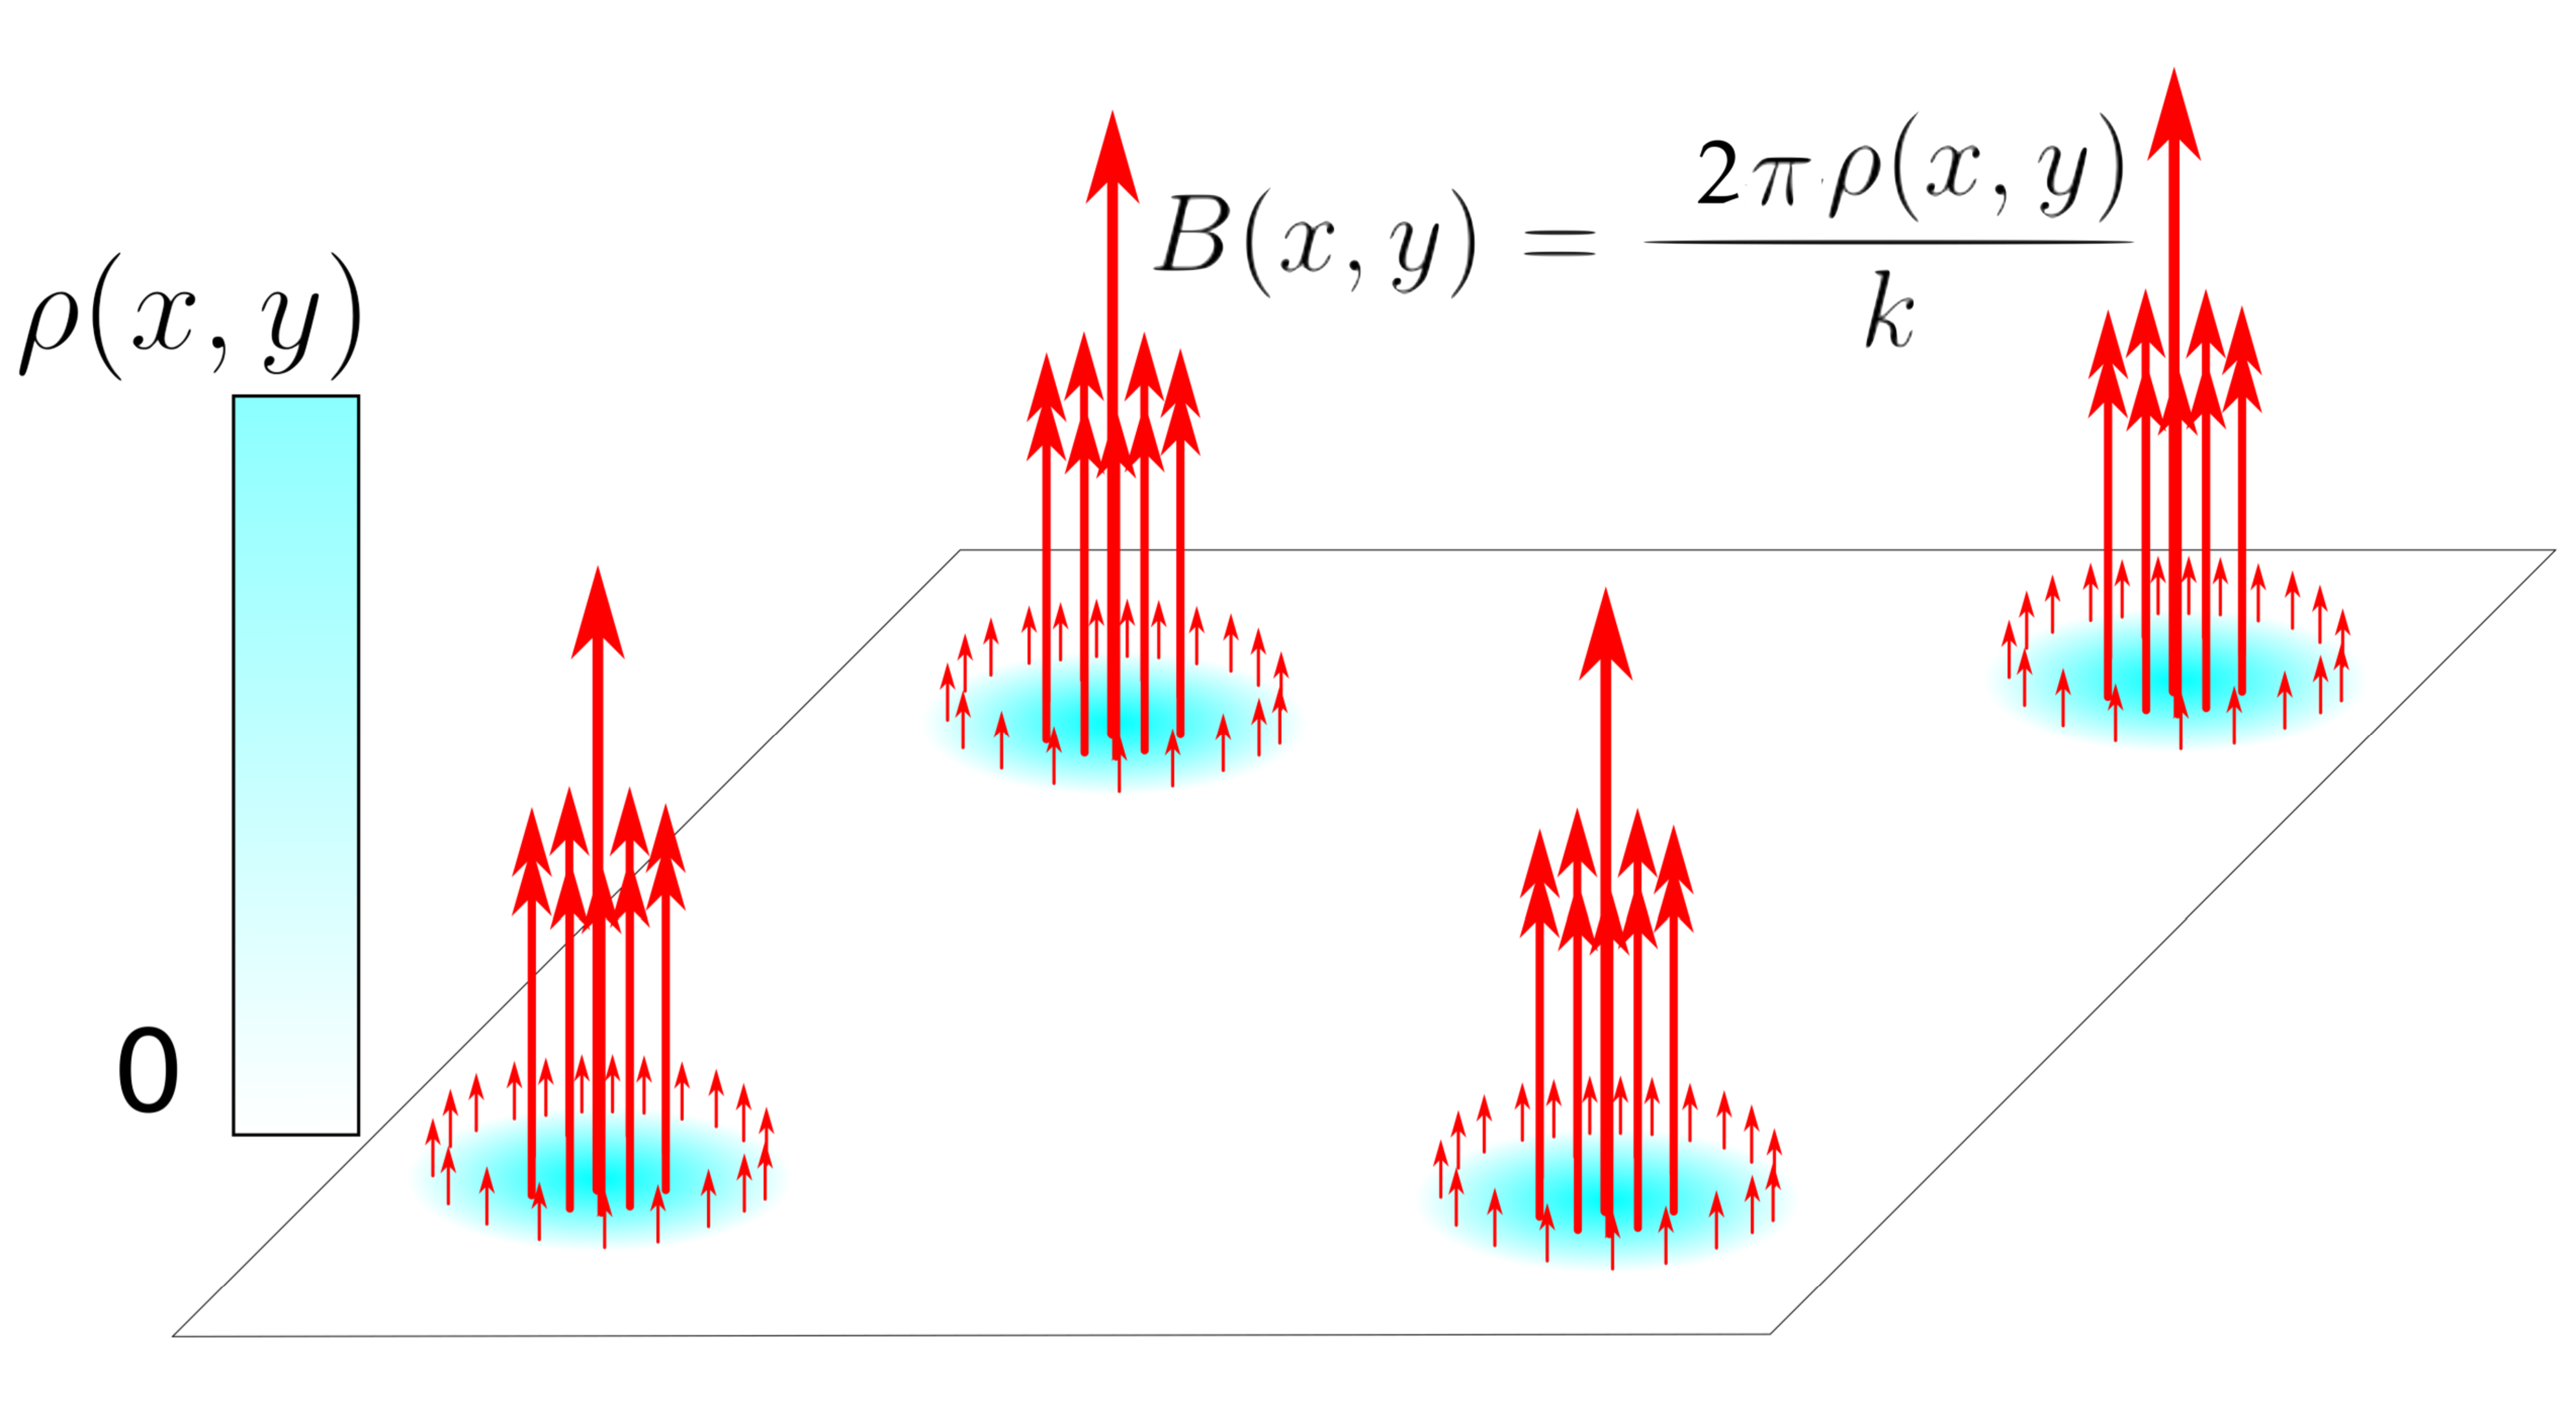
\includegraphics[scale=0.17]{Background_Folder/figures/Flux_Attachment_3.pdf}
    \caption[This figure depicts magnetic flux attachment.]{A collection of locali\textcolor{red}{s}ed charge distributions, and with magnetic flux lines of strength $\frac{\textcolor{red}{2} \pi \rho(x,y)}{k}$ tied to the charges. Here the charge density distribution is denoted by $\rho(x,y)$ and the magnetic field strength is denoted by $B(x,y)$. Darker shades of cyan depict a larger charge density and larger red vectors are associated with a stronger magnetic field perpendicular to the plane.  The charge and flux are tied together throughout the motion of the particles as a result of the Chern-Simons equations \eqref{eq:source_abel_charge} - \eqref{eq:source_abel_current}.} \label{fig:flux_attachment}
\end{figure}

The final aspect of Chern-Simons theory that we will use is the fact that it is a \textit{topological} field theory (TQFT). This means that the theory is independent of the metric. This consequently implies that the CS term does not contribute to the energy-momentum tensor, since
\begin{align}
    T^{\mu \nu} = \frac{-2}{ \sqrt{-g}} \frac{\delta S_{\text{CS}}}{ \delta g_{\mu\nu}} =0.
\end{align}

One way to see that CS is a topological field theory is by writing it as an integral of a differential form
\begin{align}
    S_{\text{CS}} &= \frac{k}{4 \pi} \int \left(A \wedge dA +A \wedge A \wedge A\right).
\end{align}
This construction does not require the metric to be defined, unlike the Yang-Mills term, which involves the Hodge star (a metric dependent construct) in order to be defined through differential forms.

This concludes our review of CS theory. We now move on to a refresher of statistical physics.


        \section{Statistical Physics}

        Here we motivate the study of QFT as a gateway into understanding phenomena in many body physics. Physical phenomena at macro scale require micro scale explanations. The transition between a microscopic theory and its observable large scale properties is facillitated by the use of techniques in statistical mechanics. Here we review the connection between microscopic Lagrangian formulation and the statistical partition function through the formalism of the path integral. We follow through by accentuating the treatment of a chemical potential and the subtleties related to it. Before we go on, I note that this is the only part of this section that will be relevant to the calculations performed in this work. However, the rest of this section is meant to shine a light on why it is that we are interested in such an abstract problem.

        Upon completing this summary, we go through a short review of statistical mechanical paradigms, their successes and shortcomings. In particular, we will highlight how the Landau-Fermi liquid theory \cite{Landau:1956zuh} manages to do away with the complications arising from interactions and how succesful the Landau-Ginzburg symmetry breaking ideas have been in explaining large swathes of interesting phases of matter. 

        Finally, the failures of these extremely successful ideas will lead us to strongly correlated and topological systems. Notably, we discuss one system that seems to reject treatment from both of the above approaches -- a system of strongly interacting electrons confined to 2 dimensions, namely, the physical setup in which we observe the Quantum Hall effect. As the reader might suspect, the planar confinement is what forces us into considering CS theory as a natural candidate to explain the exotic properties of this structure.
        \subsection{Functional \textcolor{red}{i}ntegral \textcolor{red}{r}epresentation of the \textcolor{red}{p}artition \textcolor{red}{f}unction}
        In this section we derive the functional integral representation of the partition function for interacting relativistic non-gauge field theories. Good reviews on the techniques we discuss here can be found in \cite{Laine:2016hma, 0486477223}.
        Let $\hat{\phi}(\bm{x},0)$ be a Schr{\H o}dinger picture field operator at time $t=0$. We define its conjugate momentum operator to be $\hat{\pi}(\bm{x},0)$. The eigenstates of the field operator are labe\textcolor{red}{l}led $| \phi \rangle$ and satisfy
        \begin{align}
            \hat{\phi}(\bm{x},0) | \phi \rangle = \phi(\bm{x}) | \phi \rangle,
        \end{align}
        where $\phi(\bm{x})$ is the eigenvalue of $| \phi \rangle$. This is complemented with the completeness and orthogonality relation
        \begin{align}
            \int d \phi(\bm{x}) | \phi \rangle \langle \phi | = 1, \\
            \langle \phi_a | \phi_b \rangle = \prod_{\bm{x}} \delta(\phi_a(\bm{x}) - \phi_b(\bm{x})).
        \end{align}
        And similarly for the conjugate momentum
        \begin{align}
            \hat{\pi}(\bm{x},0) | \pi \rangle = \pi(\bm{x}) | \pi \rangle, \\
            \int d \pi(\bm{x}) | \pi \rangle \langle \pi | = 1, \\
            \langle \pi_a | \pi_b \rangle = \prod_{\bm{x}} \delta(\pi_a(\bm{x}) - \pi_b(\bm{x})).
        \end{align}
        Suppose we have a Hamiltonian with no explicit time dependence
        \begin{align}
            H = \int d^2x \, \mathcal{H}(\hat{\phi}, \hat{\pi}).
        \end{align}
        Assume that a system is in a state $| \phi_a \rangle$ at time $t=0$. After a time $t_f$ it evolves to $e^{-i H t_f} | \phi_a \rangle$, assuming that the Hamiltonian has no explicit time dependence. The transition amplitude for going from state $| \phi_a \rangle$ to state $| \phi_b \rangle$ after a time $t_f$ is $\langle \phi_b | e^{-i H t_f} | \phi_a \rangle$. In order to study a system at thermodynamic equilibrium, we will be interested in the amplitude for the system returning to the same state after a time $t_f$. To be able to compute this amplitude, we divide the time interval $(0, t_f)$ into $N$ equal time steps $\Delta t = \frac{t_f}{N}$. Then at each time interval, we insert a complete set of states, alternating between field operators and their conjugate momenta


        \begin{align}
            \langle \phi_a| e^{- i H t_f} | \phi_a \rangle &= \lim_{N\rightarrow \infty} \int \left( \prod_{i=1}^{N} \frac{d\pi_i d\phi_i}{2\pi} \right) \nonumber \\
            &\times \langle \phi_a | \pi_N \rangle \langle \pi_N|  e^{-i H \Delta t}| \phi_N \rangle \langle \phi_N | \pi_{N-1} \rangle \nonumber \\
            &\times \langle \pi_{N-1} | e^{-i H \Delta t} | \phi_{N-1} \rangle \dots \nonumber \\
            &\times \langle \phi_2 | \pi_1 \rangle \langle \pi_1 | e^{-i H \Delta t} | \phi_1 \rangle \langle \phi_1 |\phi_a \rangle.
        \end{align}
        In order to evaluate this expression, we need to do several things. First of all, from single particle QM, we know that 
        \begin{align}
            \langle x | p \rangle = e^{i p \cdot x}.
        \end{align}
        So an appropriate generalization for this inner product to field operators is 
        \begin{align}
            \langle \phi_{i+1}| \pi_i \rangle = \exp \left(i \int d^2 x \ \pi_i(\bm{x}) \phi_{i+1}(\bm{x}) \right).
        \end{align}
        Since $\Delta t \rightarrow 0$, we can expand as follows, keeping terms up to first order:
        \begin{align}
            \langle \pi_i | e^{-i H_i \Delta t} | \phi_i \rangle &\sim \langle \pi_i | (1- i H_i \Delta t ) | \phi_i \rangle \nonumber \\
            &= \langle \pi_i | \phi_i \rangle (1 - i H_i \Delta t) \nonumber \\
            & = (1-i H_i \Delta t) \ \exp\left(-i \int d^2x \, \pi_i(\bm{x}) \phi_i (\bm{x})  \right),
        \end{align}
        where
        \begin{align}
            H_i = \int d^2 x \ \mathcal{H}\left(\pi_i (\bm{x}) \phi_i (\bm{x}) \right).
        \end{align}
        In the end we arrive at 
        \begin{align}
            \langle \phi_a | e^{-i H t_f} | \phi_a \rangle &= \lim_{N\rightarrow \infty} \int \left( \prod_{i=1}^N \frac{d \pi_i d\phi_i}{2\pi} \right) \delta \left(\phi_1 -\phi_a \right) \nonumber \\
            &\times \exp \left(i \Delta t \sum_{j=1}^{N} \int d^2x \left[\frac{\pi_j (\phi_{j+1} -\phi_j)}{\Delta t} - \mathcal{H}(\pi_j, \phi_j) \right] \right).
        \end{align}
        And taking the continuum limit we arrive at the path integral representation of the partition function
        \begin{align}
            &\langle \phi_a | e^{-i H t_f} | \phi_a \rangle = \int \mathcal{D} \pi \int_{\phi(\bm{x},0) =\phi_a(\bm{x})}^{\phi(\bm{x}, t_f) = \phi_a(\bm{x})} \mathcal{D} \phi \nonumber \\
            &\times \exp \left[i \int_0^{t_f} dt \int d^2 x \left( \pi(\bm{x} ,t) \frac{\partial\phi(\bm{x}, t)}{ \partial t} - \mathcal{H}\left(\phi(\bm{x},t), \pi(\bm{x},t)\right) \right) \right] \label{eq:path_integral_amplitude}.
        \end{align}
        For a Hamiltonian that is quadratic in the canonical momenta, we can just complete the square, integrate out the momenta and arrive at the usual expression for a transition amplitude in terms of a path integral over $e^{i S}$. Since our purpose here is to illuminate the connection between the statistical partition function and the path integral, we shall perform a few more manipulations. 
        \subsection{Grand \textcolor{red}{c}anonical \textcolor{red}{e}nsemble} \label{GCE_sec}
        First, we note that the grand canonical partition function is defined as follows
        \begin{align}
            Z= \textcolor{red}{\mathrm{Tr}} \left[e^{-\beta \left( H - \mu N \right)}\right],
        \end{align}
        where $\beta = \frac{1}{k_b T}$ and is the inverse temperature and $\mu$ is the \textit{chemical potential}, and $N$ is a particle number. In a QFT this particle number will be associated with a conserved charge that is discreti\textcolor{red}{s}ed, which is the reason why it is associated to particle number. We can express the trace in the $\phi$ basis
        \begin{align}
            Z= \int d \phi_a \langle \phi_a | e^{-\beta \left( H - \mu N \right)} | \phi_a \rangle.
        \end{align}
        We see that this expression is very similar to \ref{eq:path_integral_amplitude}. In order to match the two expressions, we need to do three things. First, we set $t \rightarrow -i \tau$, such that $t_f \rightarrow -i \beta$. Then we shift the Hamiltonian density in order to account for the inclusion of a chemical potential
        \begin{align}
            \mathcal{H} \left(\phi(\bm{x},t),\pi (\bm{x},t) \right) \rightarrow \mathcal{H}\left(\phi(\bm{x},t),\pi (\bm{x},t) \right) - \mu \ \mathcal{N}\left(\phi(\bm{x},t),\pi (\bm{x},t) \right),
        \end{align}
        where $\mathcal{N}$ is a number density. Finally, we include the trace operation, which integrates over all possible boundary conditions. In the end we are left with
        \begin{align}
            Z &= \int \mathcal{D} \pi \int_{\text{periodic}} \mathcal{D} \phi \exp \left[ \int_0^{\beta} \int d^2x \left(\pi \frac{\partial \phi}{\partial t} - \mathcal{H}(\pi, \phi) + \mu \mathcal{N}(\pi, \phi) \right) \right] \label{eq:partition_function}.
        \end{align}
This is the path integral representation of the partition function of the grand canonical ensemble of a single real scalar field. This expression is readily generalizable to more fields by integrating over the extra fields and their respective conjugate momenta.

Here we shall make a few observations that will come in use frequently for the rest of this work. For the purposes of presentation, we will elaborate on these points in the context of a somewhat simpler model. This should not alarm the reader, because the properties we are discussing are more general and model independent. With this in mind, we consider the Lagrangian description of a complex relativistic scalar in $2+1d$ with a potential $U(\phi)$
        \begin{align}
            \mathcal{L} = \left(\partial_{\mu}\phi^{*} \partial^{\mu} \phi  - U\big(|\phi|\big)\right).
        \end{align}
        This system possesses a global symmetry
        \begin{align}
            \phi \rightarrow e^{i \alpha} \phi, \qquad\qquad \phi^* \rightarrow e^{-i \alpha} \phi^*.
        \end{align}
        This leads to a conserved Noether current and consequently a conserved charge
        \begin{align}
            J_{0} &= -i \int d^2x \left( \pi \phi - \pi^{\dag}\phi^{\dag}\right),
        \end{align}
        where $\pi = \frac{\delta \mathcal{L}}{\delta ( \partial_0 \phi)}$ is the canonical momentum. Based on the assumption of identical particles with discrete charges, we postulate that $J_0 = \mathcal{N}$. Next, we perform the momentum integrals in \eqref{eq:partition_function}. Since now we have a complex field, we have to integrate over all of $\phi$, $\phi^{\dag}$, $\pi$ and $\pi^{\dag}$
        \begin{align}
            Z &= \int \mathcal{D} \pi \mathcal{D} \pi^{\dag} \int_{\text{periodic}} \mathcal{D} \phi \mathcal{D} \phi^{\dag} \nonumber \\
            &\times \exp \left[ \int_0^{\beta} \int d^2x \left(\pi \frac{\partial \phi}{\partial t} +\pi^{\dag} \frac{\partial \phi^{\dag}}{\partial t} - \mathcal{H}(\pi, \pi^{\dag}, \phi, \phi^{\dag}) - i  \mu \left(\pi \phi - \pi^{\dag}\phi^{\dag} \right) \right] \label{eq:partition_function_complex_scalar} \nonumber \\
            &= \int \mathcal{D} \pi \mathcal{D} \pi^{\dag} \int_{\text{periodic}} \mathcal{D} \phi \mathcal{D} \phi^{\dag} \nonumber \\
            &\times \exp \left[ \int_0^{\beta} \int d^2x \left(\pi \left( \frac{\partial \phi}{\partial t} -i \mu \phi \right) +\pi^{\dag} \left( \frac{\partial \phi^{\dag}}{\partial t} +i \mu \phi^{\dag} \right) - \mathcal{H}(\pi, \pi^{\dag}, \phi, \phi^{\dag}) \right) \right]. \label{eq:partition_function_complex_scalar}
        \end{align}
        Performing the path integral leaves us with
        \begin{align}
            Z= \int_{\text{periodic}} \mathcal{D}\phi \mathcal{D}\phi^{\dag} \exp \left[\int_0^{\tau} d\tau \int d^2x \mathcal{L'} \right],
        \end{align}
        where $\mathcal{L'}$ is the same as $\mathcal{L}$ except for the time derivatives acting on $\phi$ now act as covariant derivatives in the presence of a constant background gauge field $A_0=\mu$, \ie
        \begin{align}
            \partial_0 \rightarrow \partial_0 -i \mu. \label{eq:chemical_potential_gauge_field}
        \end{align}
        This is a general result that we will be making use of numerous times.
        \subsubsection{Chemical \textcolor{red}{p}otential for a \textcolor{red}{l}ocal \textcolor{red}{s}ymmetry}
        Now, let us see how this situation changes when we try to introduce a chemical potential for a gauged symmetry. First, we modify the Lagrangian $\mathcal{L}$ by gauging the $U(1)$ and adding a Maxwell term $-\frac{1}{4 g^2} F_{\mu \nu} F^{\mu \nu}$. For simplicity, let us assume that the potential has the monomial super-renormalizable form
        \begin{align}
            U\big(|\phi| \big) = \lambda |\phi|^4.
        \end{align}
        Therefore
        \begin{align}
            \mathcal{L} &=( D_{\mu} \phi)^* D^{\mu} \phi - \lambda |\phi|^4 - \frac{1}{4 g^2}F_{\mu \nu} F^{\mu \nu},
        \end{align}
        where $D_{\mu}= \partial_{\mu} - i A_{\mu}$. According to the rule \ref{eq:chemical_potential_gauge_field} that we established above,
        \begin{align}
            \mathcal{L} \rightarrow \mathcal{L}'= \mathcal{L}\left(\phi,\ D_{\mu}' \phi,\ A_{\mu} \right),
        \end{align}
        where $D_{\mu}' = D_{\mu} - i \mu \delta_{\mu 0}$.
        Let us also express $\phi$ in terms of a modulus and a phase
        \begin{align}
            \phi(x) = \sigma(x) e^{i \alpha(x)}.
        \end{align}
        If we assume a homogenous, constant configuration, the equations of motion tell us that
        \begin{align}
            \sigma &= \sqrt{\frac{\mu^2}{2\lambda}}  \label{eq:chem_pot_local_symmetry_eom1}, \\
            \frac{1}{g^2} \partial_{\mu} F^{\mu 0} &= \mu \sigma^2. \label{eq:chem_pot_local_symmetry_eom2}
        \end{align}
        The first equation tells us that the scalars have condensed to the ground state. The second equation states that we have a non-zero charge density in this ground state. On the one hand, this makes sense, since the charged scalars have condensed. On the other hand, this is contradictory, since we are studying a system at equilibrium. And a charged system cannot be in equilibrium by definition. In order to fix this problem, we introduce a background charge density, which guarantees that the system is neutral 
        \begin{align}
            \mathcal{L}' \rightarrow \mathcal{L}' - A_0 J_0,
        \end{align}
        where $J_0 = \frac{\mu^3}{2\lambda}$.

        %\subsection{Physical Applications}\label{phys_app_sec}
        %\subsubsection{Landau-Fermi Liquid Theory} \label{Fermi_Liquid_sec}
        The statistical description of weakly interacting particles, for example, in a fluid can be thought of as the same as that of a free gas of non-interacting quasiparticles that are in one to one correspondence with the original interacting excitations of the material. We find that in order to explain some of the surprising feature of the charge carriers in a QH system, we need to go beyond the weakly interacting description of a Landau-Fermi liquid.
        %\subsubsection{Landau-Ginzburg Paradigm} \label{Landau-Ginzburg_sec}
        %\textcolor{red}{***More to add***} \\
        %- Introductory part talk about the problem of scales, how mean field theory tackles the problems well away from the critical temperature, but at the critical point, all scales need to be taken into account. We are left with a LG functional that no longer contains information about the microscopic system -- we find a universal effective theory describing said phenomenon.
        %- Symmetry breaking \\
        %- Order parameters\\
        %- The Girvin MacDonald ``Landau-Ginzburg''-like model. \cite{Girvin1987} In 1987, Girvin \& MacDonald proposed a LG effective model to describe the FQHE. \\
        %- Read's improvement \cite{Read1989}\\
        %- The Zhang, Hansson, Kivelson microscopic Hamiltonian improvement \cite{PhysRevLett.62.82}
        \section{Fractional Quantum Hall Effect} \label{FQHE_sec}
        Here we discuss what is perhaps the most applied aspect of TQFT in the real world. But before we get to the point of discussing the highly non-trivial physics of the various types of \textcolor{red}{q}uantum Hall \textcolor{red}{e}ffects, we take a moment to review the classical picture.
        \subsection{Classical Hall \textcolor{red}{e}ffect}
        In the year 1879, \textit{Edwin Hall} \cite{Hall1879} set up an experiment consisting of a conductor plate with two electrodes attached at either end of it, generating a current, and a magnetic field penetrating the surface of the conductor perpendicularly. He found that he could measure a non-zero potential across the conductor, orthogonal to the plane defined by the driving current and the magnetic field. The generation of this potential difference has since been known as the \textit{Hall effect}. Despite this being an exciting discovery at the time, from our modern perspective this is all accounted by basic knowledge of conductors and classical electrodynamics. In the presence of a magnetic field, the charge carriers, which are responsible for the current in the conductor, get deflected in a direction orthogonal to their motion due to the Lorentz force
        \begin{align}
            F = q(\bm{E} + \bm{v}\times \bm{B}),
        \end{align}
        where $q$ is the charge of the electrons, $\bm{E}$ is the electric field due to the potential difference in the electrodes, $\bm{v}$ is the velocity of the charge carriers and $\bm{B}$ is the magnetic field in the material. If we were to account for the possible collisions that may occur within a sample of the conductor, which will cause the charge carriers (in this case electrons) to slow down, we shall arrive at a slightly modified equation to the Lorentz law from above
        \begin{align}
            m \dot{\bm{v}} = q \bm{E}+q \bm{v}\times \bm{B} - \frac{1}{\tau} m \bm{v}, \label{eq:Drude_Model_Background}
        \end{align}
        where $\tau$ is the \textit{scattering time} -- it accounts for how frequently the electrons scatter, hence a large scattering time makes the term disappear completely. This description of the charge carriers in a material, subject to both electric and magnetic field, in the presence of impurities, is called the \textit{Drude model}, named after the German physicist \textit{Paul Drude}, who first proposed it \cite{Drude1900a, Drude1900b}. Before we look at the general solution of this model, we make several remarks about certain limiting cases.\\
        \indent First, assume that there are no collisions (\textit{i.e.} the collision time diverges $\tau \rightarrow\infty$) and that there is no electric field. Then the system simplifies to
        \begin{align}
            m\dot{\bm{v}} =q \bm{v}\times \bm{B}.
        \end{align}
        For a particle confined to the plane the velocity vector is $\bm{v} = (\dot{x}, \dot{y})$, which leads to the system of two coupled linear ODEs
        \begin{align}
            m \ddot{x} = q B \dot{y}, \qquad m \ddot{y}= -q B \dot{x}.
        \end{align}
        The general solution to this system is
        \begin{align}
            x(t) &= x_0 + R \sin\left(\omega_Bt + \varphi \right), \\
            y(t) &= y_0 + R \cos\left(\omega_Bt + \varphi \right),
        \end{align}
        where $x_0, y_0, R, \varphi$ are all integration constants and
        \begin{align}
            \omega_B = \frac{q B}{m}
        \end{align}
        is the \textit{cyclotron frequency}.
        We \textcolor{red}{see} that the solution in the absence of collisions and an electric potential is circular motion with a fixed magnetic field dependent frequency \textcolor{red}{$\omega_B$}.

        Let us go back to the full Drude model. We would like to find out what the equilibrium of the system looks like. This implies that $\dot{v} =0$. The equation of motion becomes 
        \begin{align}
            \bm{v} - \frac{q \tau}{m}\bm{v}\times\bm{B}  &=\frac{\tau q}{m} \bm{E} ,\\
            \begin{bmatrix}
                1 & -\frac{q \tau B}{m} \\
                \frac{q \tau B}{m} & 1 \\
            \end{bmatrix} \bm{v} &= \frac{\tau q}{m} \bm{E}.
        \end{align}
        Subsituting $\bm{J} = q \bm{v}$ and $\omega_B = \frac{q B}{m}$
        \begin{align}
            \begin{bmatrix}
                1 & -\omega_B \tau \\
                \omega_B \tau & 1 \\
            \end{bmatrix}\bm{J} = \frac{\tau q^2}{m} \bm{E}.
        \end{align}
        After inverting we arrive at \textit{Ohm's law}
        \begin{align}
            \bm{J}=\sigma \bm{E}, \label{Ohms_Law}
        \end{align}
        where
        \begin{align}
            \sigma=\frac{q^2 \tau }{m \left(\tau ^2 \omega_B ^2+1\right)}
\begin{bmatrix}
 1 & \tau  \omega_B  \\
 -\tau  \omega_B  & 1 \\
\end{bmatrix}
        \end{align}
         is the \textit{conductivity} tensor. It is related to the \textit{resistivity} tensor by \textcolor{red}{inversion}
         \begin{align}
            \rho = \sigma^{-1}= \frac{m}{q^2 \tau } \begin{bmatrix}
 1 & -\tau  \omega_B  \\
 \tau  \omega_B  & 1 \\
            \end{bmatrix} = \begin{bmatrix}
                \rho_{xx} & \rho_{xy} \\
                \rho_{yx} & \rho_{yy} \\
            \end{bmatrix},
         \end{align}
         where $\rho_{xx} =\rho_{yy}$ and $\rho_{xy} = - \rho_{yx}$.

         This equation tells us that in the presence of a constant magnetic field, the charge carriers experience two types of resistivity. One is the usual type of resistivity that you can expect from a conductor $\rho_{xx} = \frac{m}{q^2\tau}$ -- \textcolor{red}{i}t is independent of the magnetic field and as the scattering time increases, \textit{i.e.} the number of scattering events decreases, the resistivity decreases. The other type of resistivity is different. The off-diagonal component of the resistivity $\rho_{yx} = \frac{m \omega_B}{q^2}= \frac{B}{q}$ is independent of $\tau$. So somehow the resistivity in the direction orthogonal to that of the driving current does not depend on the impurities in the material. Another way in which $\rho_{yx}$ is different is that it depends on the magnetic field. Surprisingly, as $B\rightarrow 0$ so does $\rho_{yx} \rightarrow 0$. It would be incorrect to assume that the vanishing of $\rho_{xy}$ implies that we achieve superconductivity, since $\sigma_{xy}$ also vanishes so there is no current being generated perpendicular to the generating electric field.

        The Drude model is successful when compared to the classical experimental results obtained by Hall since it predicts correctly that the resistivity  $\rho_{xy}$ would grow linearly with the magnetic field $B$.
        \subsection{Quantum Hall \textcolor{red}{e}ffect}
        Now that we have an understanding of the classical Hall effect we are ready to delve into the physics of the \textcolor{red}{q}uantum Hall effect. It's important to distinguish two different types of \textcolor{red}{q}uantum Hall effects, since they are qualitatively different, occur in different materials and seem to have fundamentally different physical explanations.
        The first type is the \textit{integer quantum Hall effect (IQHE)}. In 1980, \textit{Klaus von Klitzing et. al.} \cite{vonKlitzing:1980pdk} performed the Hall experiment at ultralow temperatures with strong magnetic fields and found that the above relation between $\rho_{yx}$ and $B$ does not hold for large enough magnetic fields. They found that beyond a certain magnetic field strength, plateaux started appearing in the resistivity that could not be explained by the classical picture. Further, they found that in the plateaux, where $\rho_{yx}$ was constant, $\rho_{xx}$ was vanishing. The precise relation that he discovered was
        \begin{align}
            \rho_{yx} = \frac{2 \pi \hbar}{e^2} \frac{1}{\nu}, \qquad \nu \in \mathbb{Z}.
        \end{align}
        Thus the quantity $\frac{2 \pi \hbar}{e^2}$ is dubbed the \textit{quantum of resistivity}. The explanation of the \textcolor{red}{i}nteger \textcolor{red}{q}uantum Hall effect is based on the quantum mechanics of non-interacting particles confined to a plane. In the case of the fractional \textcolor{red}{q}uantum Hall effect (FQHE), where $\nu \in \mathbb{Q}$, we need to study a highly interacting system, which makes the FQHE a very interesting topic for theoretical physics.

 \textcolor{red}{\subsection{Landau levels and the integer quantum Hall effect.}}

\textcolor{red}{Before we attempt to tackle the intricacies of the FQHE, we will have to first acquaint ourselves with the quantum mechanical analogue of the Drude model. Namely, we will be interested in the quantum mechanics of a charged particle, confined to a plane, subjected to a magnetic field perpendicular to that plane (For now we will consider the electric field to be vanishing). The physics of this system can be described by a harmonic oscillator. The energy states of this system are today referred to today as \textit{Landau levels}. The name comes from Landau's description of diamagnetism in metals through the quanti\textcolor{red}{s}ed orbits of free electrons in a metal \cite{Landau1930}. Historically, there have been others \cite{Rabi1928, Fock1928, FrenkelBronshtein1930}, who have either predated or have independently studied this system, but Landau's name ended up being attached to it, likely because none of the other works found the number of states or found a connection between the oscillations and the diamagnetism of metals \cite{shifman2013under}.}

\textcolor{red}{For the purpose of quantisation, we shall consider the particle in a magnetic field system in the Hamiltonian formulation. The general Hamiltonian for a particle at position $\bm{x}$ in a vector potential $\bm{A}$ is }
\begin{align}
    H=\frac{1}{2m}\left(\bm{p} +e \bm{A} \right)^2.
\end{align}

 \textcolor{red}{Here we take the special case of a vector potential such that $\nabla \times \bm{A} = B \hat{\bm{z}}$.}

\textcolor{red}{In order to solve the quantum system, we follow canonical quantization and we promote the position and momenta to operators}
\begin{align}
    \textcolor{red}{[\hat{x}_i, \hat{p}_j] = i \hbar \delta_{ij}, \qquad [\hat{x}_i, \hat{x}_j]=[\hat{p}_i, \hat{p}_j]=0.}
\end{align}

\textcolor{red}{Here we shall use \textit{Landau gauge}}

\begin{align}
    \textcolor{red}{\bm{A}=  x B\hat{y}.}
\end{align}

 \textcolor{red}{Now we can define raising and lowering operators }
\begin{align}
    \textcolor{red}{\hat{a}^{\dagger}= \hat{p}_x +i (\hat{p}_y +e A_y), \qquad \hat{a}= \hat{p}_x  -i (\hat{p}_y +e A_y).}
\end{align}
 \textcolor{red}{Substituting the form of $A$ in Landau gauge and using the canonical quantization conditions, we get the usual commutation relations}
\begin{align}
    \textcolor{red}{ [\hat{a}, \hat{a}^{\dagger}] =1.}
\end{align}

 \textcolor{red}{ In terms of $\hat{a}$ and $\hat{a}^{\dagger}$, the Hamiltonian takes the standard form}

\begin{align}
    \textcolor{red}{ H = \hbar \omega_B \left( \hat{a}^{\dagger} \hat{a}+ \frac{1}{2}\right),}
\end{align}

 \textcolor{red}{ where $\omega_B=\frac{eB}{m}$. This leads to a tower of energy eigenstates $|n\rangle$ with energies}
\begin{align}
    \textcolor{red}{ E_n= \hbar \omega_B \left( n + \frac{1}{2} \right), \qquad n \in \mathbb{N}.}
\end{align}
 \textcolor{red}{ Since we are studying the QHE, we expect the magnetic fields to be large, hence the gap between the energy levels would appropriately be very large too. If the gap is in addition very large in comparison to the temperature of the system, \textit{i.e.} $k_B T \ll \hbar \omega_B$, then we expect that only the first few Landau levels would be occupied. An important fact to take note of here is that we are attempting to study a system of a macroscopic number of electrons, yet we see that they occupy only a few energy states. This tells us that these energy eigenstates are extremely degenerate. This degeneracy is what is going to play a role in the conductivity computation.}

 \textcolor{red}{ Let us extend this to include an electric field. We choose the direction of the electric field to be in the $x$ direction, which results in an electric potential $\phi = -Ex$.}
\begin{align}
    \textcolor{red}{ H=\frac{1}{2m}\left(\bm{p} +e \bm{A} \right)^2 -e Ex.}
\end{align}
 \textcolor{red}{ The current of a particle is given by}
\begin{align}
    \textcolor{red}{ {\bf{I}}=-e\dot{{\bf x}}=  \dot{{\bf x}}= \frac{\left({\bf p}+e{\bf A}\right)}{m}.}
\end{align}
 \textcolor{red}{ Quantum mechanically, we need to average over the available charge carriers. If we are working in the $k_b T \ll \hbar \omega_B$ limit, then only the first $\nu$ Landau levels contribute, so we have}
\begin{align}
    \textcolor{red}{ \langle {\bf I} \rangle = - \frac{e}{m} \sum_{n=1}^{\nu} \sum_{k}  \langle \psi |-i \hbar \nabla +e \bf{A} |\psi \rangle.}
\end{align}
 \textcolor{red}{ The current in the $x$ direction is }
\begin{align}
    \textcolor{red}{ I_x = -\frac{e}{m} \sum_{n=1}^{\nu} \sum_{k} \langle \psi|p_x | \psi \rangle=0,}
\end{align}
 \textcolor{red}{ which vanishes since it averages $p_x$ over harmonic oscillator eigenstates. The current in the $y$ direction is}
\begin{align}
    \textcolor{red}{ I_y = e \nu \sum_{k} \frac{E}{B}.}
\end{align}
 \textcolor{red}{ Assuming that the Landau levels are completely filled, which would be the case if the \textit{Fermi energy} is in the gap between the levels, the sum over $k$ is the number of electrons per Landau level. The number of electrons per Landau level can be approximately derived by taking a unit area $A$ and dividing it by the size of an electron orbit $2 \pi l_B^2$ }
\begin{align}
    \textcolor{red}{ \sum_{k}1 = N = \frac{A B e}{2 \pi \hbar}.}
\end{align}
 \textcolor{red}{ This leaves us with the \textit{current density}}
\begin{align}
    {\bf J} = \begin{pmatrix} 
0\\
        \frac{-e^2 \nu E}{2 \pi \hbar}
    \end{pmatrix}.
\end{align}
 \textcolor{red}{ We can again use Ohm's law (\ref{Ohms_Law}) and infer the conductivity tensor}
\begin{align}
    \sigma = \begin{pmatrix}
        0&\frac{- e^2 \nu }{2\pi \hbar}\\
        \frac{- e^2 \nu }{2\pi \hbar}&0
    \end{pmatrix}.
\end{align}

 \textcolor{red}{ Inverting this expression and reading the off-diagonal term we find the \textit{Hall resistivity} }
\begin{align}
    \textcolor{red}{ \rho_{xy} = - \frac{2 \pi \hbar}{e^2 \nu}.}
\end{align}


 \textcolor{red}{The above discussion shows that the IQHE effect comes out of simple quantum mechanics. We have omitted a lot of details and intricacies relating to impurities in the sample, edge states \cite{PhysRevB.25.2185}, the role of extended states and the irrelevance of locali\textcolor{red}{s}ed states \cite{PhysRevB.23.5632}, the role of topology and much more. We refer the reader to the following reviews \cite{hep-th/0509216, yoshioka2002the, Girvin} to learn more about these details. The main point that we'd like to make here is that the IQHE can be understood in terms of a non-interacting system of electrons. This is in contrast to our current understanding of the FQHE, which requires strongly interacting electrons.}


 \textcolor{red}{\subsection{Fractional quantum Hall effect}}

 \textcolor{red}{Despite the fact that a Nobel prize had already been awarded for the IQHE, a second QHE Nobel prize\footnote{https://www.nobelprize.org/prizes/physics/1998/summary/} was awarded to \textit{Laughlin, Störmer \& Tsui} \cite{Laughlin:1983fy, PhysRevLett.48.1559} in 1998 for the discovery of the FQHE! This fact alone should signal just how distinct and important the two effects are, despite arising from a system that is classically indisinguishable. As we saw in the IQHE, there is a certain, very large, value of the magnetic field $B$, for which we would find the system completely in the lowest Landau level, due to the large energy gap $\Delta E \sim B$. Measuring the resistivity perpendicular to the external electric field, we would find it to be equal to}
\begin{align}
    \textcolor{red}{ \rho_{x y} = \frac{2\pi\hbar}{e^2},}
\end{align}
 \textcolor{red}{ which corresponds to the case $\nu=1$. Decreasing the magnetic field, we find resistances corresponding to $\nu=2,3,...$ \textit{etc.} However, in certain materials with higher electron mobility \cite{yoshioka2002the} and at lower temperatures, this pattern seems to break down. We start seeing values of the resistance that are  no longer in integer values, which are, however, still quanti\textcolor{red}{s}ed.  More specifically, they are quanti\textcolor{red}{s}ed in rational fractional values of the basic unit of resistance $\frac{2 \pi\hbar}{e^2}$, hence the name \textit{fractional}. This effect persists going the other way, in increasing magnetic field, which leads to a fractionally filled lowest Landau level. This is what \textit{Störmer, Tsui \& Gossard} \cite{PhysRevLett.48.1559} observed in 1982, when they measured the resistance for a fractional filling of $\nu=\frac{1}{3}$. It appears as though the Landau levels are only fractionally filled, yet the resistance in the direction along the electric field is still vanishing. What could be happening?}

 \textcolor{red}{It turns out that increasing the electron mobility, or equivalently, reducing the impurities in the material, allows the electrons to more freely interact \cite{PhysRevB.37.8476}. This means that our treatment from the previous section, where the electrons were thought of as non-interacting particles breaks down. In order to understand what is actually happening, we need to solve the interacting electron system. Unfortunately, this is extremely difficult, due the extremely large number of degrees of freedom. In fact, to this day, there is no known model that can explain all of the fractional values that can be observed in the FQHE. It is an unsolved problem in physics, and as such provides an exciting playground for innovation.}
 
 \textcolor{red}{It seems, however, that it is possible to write down a guess that captures the correct qualitative physics and reproduces some of the filling fractions, despite not being the exact solution to the highly interacting system. Such a well-informed guess was first written down not long after the discovery of the fractional states by \textit{Laughlin} \cite{Laughlin:1983fy} and the distinct features of this guess (such as fractional charge and anyonic statistcs, that we will get to soon) keep informing a lot of the research that is being done in the field. The wavefunction that he proposed was the following }
\begin{align}
    \psi_m(z)= \prod_{j<k} \left((z_j -z_k)^m \right) \exp\left(- \frac{1}{4}\sum\limits_{l}|z_l|^2\right),
\end{align}
where $z_j= x_j+iy_j$ the position of the $j^{th}$ electron and $m$ is an \textit{odd} natural number $m \in 2\mathbb{N}+1$. This requirement comes from the fact that we are describing electrons, which are fermions, hence we expect the wave function to be completely anti-symmetric under the exchange of any 2 of them. Since we have only made continuous changes to the system from the case of the IQHE, we expect that the number of states in the lowest Landau level to remain the same. For a unit area $A$, we have $\frac{A}{2\pi l_B^2}$ states. If we pick out any given $z_i$ from the polynomial prefactor of $\psi_m(z)$, we see that it is taken to the power of $(N-1)m$. This value is also the eigenvalue of the angular momentum operator
\begin{align}
    J = \hbar \left(z \partial_z -\bar{z} \partial_{\bar{z}}), \qquad J\psi_m(z) = \hbar (N-1)m \psi_m(z).
\end{align}
This means that we expect a single electron to occupy an area of $A= 2\pi R^2 \approx 2\pi m (N-1)l_B^2$. Substituting this into our expression for the number of Landau levels, we have
\begin{align}
    \text{Degeneracy of lowest Landau levels} = m(N-1). 
\end{align}
If we take the total number of electrons in the Laughlin wavefunction and divide it by the number of occupied states we get the filling fraction
\begin{align}
    \nu = \frac{N}{m (N-1)} \xrightarrow{N \rightarrow \infty} \frac{1}{m}.
\end{align}
We see that the Laughlin wavefunction does indeed provide an explanation for some of the filling fractions. 

One can also consider excitations above this ground state. These excitations are one of the distinctive elements of the FQH liquid, since they have very peculiar properties. They are quasi-particles in the same sense as phonons, the excitations of an atomic lattice in the \textit{Debye model} \cite{Debye1912}. In the spirit of Landau-Fermi liquid \cite{Landau:1956zuh}, one can think of them as renormali\textcolor{red}{s}ed interacting elelectrons. The first of these peculiar properties is that they have a \textit{fractional charge}, which is quite surprising, given that the fundamental particles underlying the system have a quanti\textcolor{red}{s}ed charge. These fractionally charged quasi-particles have been observed in Hall systems by \textit{de Picciotto et al} and \textit{Saminadayar et al} \cite{dePicciotto:1997qc, PhysRevLett.79.2526}.

 \textcolor{red}{The second surprising feature of these excitations is that they are an example of an exotic type of particle, which only exists in systems confined to two spatial dimensions. They are particles, whose phase under exchange is neither 1 nor -1, but somewhere in between. Under an exchange the wavefunction changes as}
\begin{align}
    \psi(x) \rightarrow e^{ i\pi  \alpha} \psi(x),
\end{align}

 \textcolor{red}{where $\alpha \in (0,1)$ is a parameter, which characterizes the statistics of particles. The value $\alpha=0 $ corresponds to bosons, while $\alpha=1$, corresponds to fermions. The quasiparticles in the Laughlin state have a statistics parameter $\alpha = \frac{1}{m}$. In other words, in terms of their statistics, these particles are somewhere between bosons and fermions.  So the name given to them is \textit{anyons}, since they can have any statistics parameter. This property seems to follow from the fractional charge, which we mentioned earlier \cite{Halperin:1983zz, Wilczek:1981du}. The existence of particles with statistics which is in between that of fermions and bosons was first speculated by \textit{Leinaas \& Myrheim} \cite{Leinaas:1977fm} and later on by \textit{Wilczek} \cite{PhysRevLett.49.957}.}

 \textcolor{red}{The idea that anyonic statistics exist in 2+1 dimensions but not in 3+1 can be understood mathematically through the Braid group \cite{PhysRevLett.52.2103, Artin1947}. However, going into the details of Braid group representations will take us too far from the main subject of our study. It suffices to say that in 3+1 spatial dimensions, the interchange of $n$ particles is governed by the symmetric group $S_n$, since any world-lines that lead to an exchange can be pulled through and unbraided. This leaves us with either the trivial representation (boson) of $S_n$ or the faithful representation (fermions). On the other hand, in 2+1 dimensions, this is not the case. In order to exchange two particles, one must move them through space-time. This movement can in general braid the world-lines of particles. This braiding has the effect of leaving a non-trivial exchange phase that is neither $1$ nor $-1$.}


\textcolor{red}{\subsection{Landau-Ginzburg and Chern-Simons theory}}


The Laughlin ground state describes a new phase of matter. One, which we refer to as \textit{fractional quantum Hall liquid}. This phase is stable for small values of $m$ and we know that for very large values of $m$ (very high magnetic fields and small temperature), the two dimensional electron liquid starts to condense into a solid crystal, known as a \textit{Wigner crystal} \cite{PhysRevLett.60.2765, PhysRev.46.1002, Wigner1938}. The fractional Hall liquid is a very special type of state of matter for several reasons. One of those reasons is that if we attempt to fit it into the accepted Landau-Ginzburg paradigm in condensed matter physics, we find that we cannot explain some of the observed states \cite{wen2004quantum}. Such attempts to describe the quantum Hall liquid were first made by \textit{Girving \& McDonald} \cite{PhysRevLett.58.1252}, who showed that the Laughlin state contains off-diagonal long range order in a non-local operator. Later on, three separate groups --  \textit{Zhang, Hansson \& Kivelsson}, \textit{Read} and \textit{Ezawa \& Iwazaki} \cite{PhysRevLett.62.82, PhysRevB.43.2637, Read1989} showed that the effective field theory describing this state involves Chern-Simons theory. It seems that the fractional quantum Hall liquid belongs to a whole new class of matter, that is not governed by the classification of its symmetries. Rather, it exhibits what is now known as topological order \cite{Wen:1995qn, TopOrderRigidStates}. Topological order is physically characteri\textcolor{red}{s}ed by a ground state degeneracy, which depends on the topology of the spatial manifold, quasiparticles with anyonic statistics and non-trivial edge states \cite{Wen:1995qn}. All abelian quantum Hall states have been classified in terms of emergent Chern-Simons gauge fields \cite{PhysRevB.46.2290}.

In 1982, Wilczek observed that a particle current coupled to a CS gauge field produced states with fractional statistics through the binding of particles to flux \cite{Wilczek:1981du}. We will show how this takes place through the \textit{Aharonov-Bohm effect} \cite{Aharonov:1959fk, PhysRevLett.5.3}. The existence of charge, implies the attachment of flux to charged particles, as we already observed in (\ref{eq:source_abel_charge}). Consider two particles of charge $1$ in some units. This means that each of them has a flux $\Phi = \frac{2\pi}{k}$ attached to them. Suppose we rotate one particle around the other by 180° and then translate the configuration back to where it was. This action is clearly equivalent to just exchanging the two particles. Whatever this does to the wavefunction, it would have to tell us what type of statistics these particles obey. Performing the aforementioned operation would lead to an Aharonov-Bohm phase in the wave function proportional to
\begin{align}
    e^{i \frac{1}{2} \oint A \cdot ds}=e^{i \frac{\Phi}{2}}= e^{i \frac{\pi}{k}},
\end{align}
where the initial factor of $\frac{1}{2}$ comes from the fact that we only went half way around the second particle. For $k=0,\infty$ (the 0 case follows from there being no flux in the first place), we have bosons and for $k=1$ we have fermions. So we see that we have found the anyons from Laughlin's ground state for finite values of the CS level $k>1$!\\
\indent Yet another feature of the quantum Hall effect pops out of Chern-Simons theory when we go back to the equation of motion (\ref{eq:source_abel_current}) for the electric field in the matter-CS section. We see the off-diagonal conductivity appearing yet again
\begin{align}
    J^{i} = \sigma_{ij}E^j,
\end{align}
where $\sigma_{xy}=\frac{k}{2\pi}$. Inverting this expression and resinstating the units of resistance $\left(\frac{\hbar}{e^2}\right)$, we recover the IQHE conductivity for integer $k$
\begin{align}
    \rho_{xy} =\frac{2\pi \hbar}{e^2 k}.
\end{align}
But how does CS recover the fractional filling if we have said that $k$ is fixed to be an integer? In order to recover the fractional fillings of the Laughlin state, we postulate the existence of emergent topological degrees of freedom $a_{\mu}$, which we describe through CS theory. Since they emerge out of the collective motions of the interacting electron system, we also expect them to couple to the familiar electromagnetic gauge field $A_{\mu}$. This leads to the effective action
\begin{align}
    S_{\text{eff}} = \int d^3x \frac{k}{4\pi} \epsilon^{\mu \nu \rho} a_{\mu} \partial_{\nu} a_{\rho} + \frac{1}{2 \pi} \epsilon^{\mu \nu \rho} A_{\mu} \partial_{\nu}a_{\rho}+ A_{\mu} J^{\mu}.
\end{align}
The equations of motion of this model lead to the relation
\begin{align}
    J^{\mu} &= \frac{1}{2\pi} \epsilon^{\mu \nu \rho} \partial_\nu a_{\rho} = \frac{1}{4\pi} \frac{1}{k} \epsilon^{\mu \nu \rho} F_{\nu \rho} \\
    &\implies J^{i} = \frac{1}{2 \pi} \frac{1}{k} \epsilon^{i j} E_{j}.
\end{align}
Again, inverting this equation and reinstating units, we get the resistivity of the Laughlin states
\begin{align}
    \rho_{xy} =k\frac{2\pi \hbar}{e^2 }, \qquad k \in \mathbb{Z}!
\end{align}
One can obtain the resistivity of any abelian Hall system by adding more of these emergent gauge fields, coupling them to each other and computing their effect on the electromagnetic background gauge field. This is done through the \textit{K-matrix} approach \cite{PhysRevB.46.2290}. Despite our understanding of the abelian system, there still remain fractional fillings that remain unexplained, such as the $\nu=\frac{5}{2}$ state \cite{Willett:1987zz}.
\textcolor{red}{An excellent review on the subject of the FQHE can be found in an article by \textit{Xiao-Gang Wen} \cite{Wen:1995qn}. Explain how Landau-Ginzburg gives the correct effective theory \cite{PhysRevLett.58.1252, Read1989, PhysRevLett.62.82, PhysRevB.43.2637}. Explain how one can classify all abelian fractional quantum Hall states with Chern-Simons theory \cite{PhysRevB.46.2290,PhysRevLett.69.953}. Mention that the picture is incomplete for the case of non-abelian quantum hall states (even denominator fractions?). Mention \textit{Wen}'s idea about Topological order \cite{TopOrderRigidStates}. Mention the hierchy of states and Jain's composite fermion as special case of FQHE. \cite{PhysRevLett.63.199, Read1994}}\\
        \indent Our exploration of the \textcolor{red}{q}uantum Hall \textcolor{red}{e}ffect will stop here. What is important to take away from this section is that the understanding of the FQHE is underlied by the study of Chern-Simons theory. Thus studying the models, that are of interest in the present work, might lead to a better understanding of the fascinating problem that is the FQHE. A further connection to this problem is provided by the non-commutative Chern-Simons theory that we explore at the end of this chapter and at the end of chapter 3. Next, we turn our attention to the study of vortices.

%\textcolor{red}{***More to add***}\\
%        - Drude Model
%        - Classical electrodynamic explanation of classical Hall effect\\
%        - Integer Quantum Hall effect \\
%   \indent         - discovered by von Klitzing\\
%        - Fractional Quantum Hall effect\\
%    \indent        - Leads to charge fractionalization\\
        %           \indent - Laughlin wave function \cite{Laughlin:1983fy}
        % Jain's generalization (Composite-fermion approach)  \cite{PhysRevLett.63.199}
        % Jain Theory of the fractional Quantum hall effect \cite{Jain:1990zz}
        % 
        % Fractional charge leads to fractional statistics according to Halperin and Wilczek \cite{Halperin:1983zz, Wilczek:1981du} (This needs more elaboration)
        % First mention of anyonic statistics \cite{Leinaas:1977fm}
        \section{Vortices} \label{vortices_sec}
        This section takes up the task of summarizing basic aspects about vortices in general and specifically in Chern-Simons matter theories.
        Vortices are locali\textcolor{red}{s}ed, exact solutions to the equations of motion \textcolor{red}{ in 2 dimensions, which interpolate between two distinct vacua.}  They may or may not be finite energy configurations.
        In 1957, \textit{Abrikosov}  showed that if the surface tension between two phases of matter (in his case those were superconducting and non-superconducting phases) is negative, then a phase transition would be accompanied by the creation of a lattice of regions, whose interiors reside in a phase different from their exteriors \cite{Abrikosov1957}. He also recogni\textcolor{red}{s}ed the similarity between these regions of non-superconductivity have with the vortices formed in superfluid helium. This similarity is due to the winding of the phase of the order parameter wave function.


        Later on, in 1973, \textit{Nielsen \& Olesen} \cite{Nielsen:1973cs} showed that a solution similar to that of Abrikosov can come about through the study of a microscopic Lagrangian, as opposed to in an effective Landau-Ginzburg description. This is the Lagrangian of the abelian Higgs model with a quartic interaction. Similar solutions have been found in the abelian Higgs model with a Chern-Simons interaction by \textit{Paul-Khare} \cite{Paul:1986ix} and in the absence of a Maxwell term by \textit{Hong-Kim-Pac} \cite{Hong:1990yh}, \textit{Jackiw \& Weinberg} \cite{Jackiw:1990aw} and \textit{Jackiw, Lee \& Weinberg} \cite{Jackiw:1990pr}.

        \subsection{Global U(1) \textcolor{red}{v}ortex}

        Now we look at the properties of these solutions more closely. Before we look at the gauge theory scenario, we focus on the simplest case of a complex massive scalar with a fourth order interaction, negative mass squared and a global $U(1)$ symmetry. \textcolor{red}{This theory is described by the continuum version of the \textit{XY model}, which leads to the \textit{Berezinskii-Kosterlitz-Thouless phase transition} \cite{Kosterlitz_1973, Berezinsky:1970fr, Berezinsky:1972rfj}, which we hinted at in the Introduction}
        \begin{align}
            \textcolor{red}{S_{\text{XY}}} &=  \left|\partial_{\mu} \phi \right|^2 + m^2 | \phi |^2 - \lambda |\phi|^4.
        \end{align}
    This \textcolor{red}{action} leads to the equations of motion
    \begin{align}
        \partial_{\mu} \partial^{\mu} \phi = m^2 \phi - 2\lambda |\phi|^2 \phi.
    \end{align}
    This system has an $S^1$ vacuum manifold, parametri\textcolor{red}{s}ed by $\phi = v e^{i \theta}$, where $\theta \in [0,2\pi)$ is the planar polar angular coordinate and $v^2 = \frac{m^2}{2 \lambda}$. We may consider a field configuration that is $\phi=0$ at the origin but approaches a different point on the vacuum manifold at spatial infinity depending on $\theta$. More precisely, we are looking at a field $\phi$ such that
    \begin{align}
        \phi \xrightarrow[]{r\rightarrow \infty} v e^{i n\theta},
    \end{align}
    where $n \in \mathbb{Z}$ in order to guarantee that the physical configuration is single-valued.
    We would like to compute the energy of such a static circularly symmetric configuration
    \begin{align}
        E= 2 \pi \int_0^{\infty} r dr \left[\lambda |\phi|^4 - m^2 |\phi|^2 + |\phi'|^2 + \frac{n^2 v^2}{r^2} \right].
    \end{align}
    Close to infinity, the potential term vanishes and so does $\phi'$. In the end we are left with
    \begin{align}
        E = 2\pi n^2 v^2 \int \frac{dr}{r} =  2\pi n^2 v^2  \ \log R,
    \end{align}
    where $R$ is the sample size on which our theory is defined. We see that the global vortex, if it exists, would only have a finite energy for finite samples and is not well-defined in the most general case. It turns out that once the global symmetry is gauged, the divergence disappears and we have a vortex configurations that is well defined in the infinite volume limit.
        \subsection{Local U(1) \textcolor{red}{v}ortex}
        The gauged $U(1)$ vortex, also known as the \textit{Abrikosov-Nielsen-Olesen vortex} is again a configuration that interpolates between two different vacua in a theory, but this time we introduce a gauge field, whose dynamics is governed by a Maxwell term and is minimally coupled to a $U(1)$ scalar with a symmetry breaking potential. This is the familiar abelian Higgs model
        \begin{align}
            S_{\text{AH}} & = \int d^3x \left[-\frac{1}{4} F_{\mu \nu} F^{\mu \nu} + | D_{\mu} \phi|^2 - U(\phi) \right], \label{eq:Abelian_Higgs_Model}
        \end{align}
        where
        \begin{align}
            U(\phi) = \frac{\lambda}{2} |\phi|^4 - m^2 |\phi|^2.
        \end{align}
    Again, we have non-trivial manifold of ground states and we can repeat the construction from above. This time the energy of the static radially symmetric configuration ends up slightly different
    \begin{align}
        E = 2 \pi \int_0^{\infty} r dr \left(\frac{1}{2}( B^2 + E^2) + |D_{\mu} \phi|^2 + U(\phi) \right) .
    \end{align}
    This time we are aiming for eliminating the divergence that arose from the kinetic term $|\partial_{\mu}\phi|$ by requiring that $A_{\mu}$ asymptotes to a value that cancels it, in such a way that this value can be arrived at through a gauge transformation, ensuring that at $r\rightarrow \infty$, $A_{\mu}$ is pure gauge, thus yielding a finite contribution from the electromagnetic field. Such a choice for $A_{\mu}$ is
    \begin{align}
        A_{\mu} = n \partial_{\mu} \alpha(x),
    \end{align}
    where $\alpha(x) = \theta$. Hence
    \begin{align}
        A_0 =0, \qquad A_r =0, \qquad A_{\theta} = n.
    \end{align}
    This implies that
    \begin{align}
        \int_0^{\infty} r dr |D_{\mu}\phi|^2 = v^2\int_0^{\infty} r dr  \frac{1}{r^2}|n-A_{\theta}|^2 =0.
    \end{align}
    From here we see that the inclusion of a gauge field has cured the divergence and we are left with a sensible infinite volume limit. \\
    \indent Now that we know that these boundary conditions do not lead to a divergence in the energy, let us see whether a solution with such boundary conditions exists. We write down the equations of motion
    \begin{align}
        \frac{1}{g^2}  \partial_{\rho}(r F^{\mu \rho}) = i r \left[\phi^* \left(D^{\mu}\phi\right) - \left(D^{\mu}\phi \right)^* \phi \right], \nonumber \\
        \partial_{\mu} \left(r D^{\mu} \phi \right) - i A_{\mu} D^{\mu} \phi + \frac{\delta U}{\delta \phi^*} =0.
    \end{align}
    After substituting the ansatz
    \begin{align}
        \phi = \sqrt{\frac{m^2}{\lambda}}v(r) e^{i n \theta}, \qquad A_{\mu} = n a(r) \delta_{\theta \mu},
    \end{align}
    and rescaling $r\rightarrow \frac{\hat{r}}{m}$, we arrive at a system of equations for the dimensionless functions $v(r)$ and $a(r)$
    \begin{align}
        \frac{1}{\hat{r}} \frac{d }{d \hat{r}} \left(\hat{r} \frac{d v}{d \hat{r}} \right) - \frac{n^2 (a-1)^2 v}{\hat{r}^2} -v^3 +v =0,  \\
        \frac{d}{d \hat{r}}\left(\frac{1}{\hat{r}}\frac{d}{d \hat{r}} a \right)- \frac{2 g^2}{\lambda r} (a-1)v^2=0.
    \end{align}
    In these variables, the boundary conditions become
    \begin{align}
        v(0) = 0, \qquad a(0)=0, \\
        v(\infty) =1, \qquad a(\infty) =1.
    \end{align}
    \textcolor{red}{Existence of a solution to non-linear boundary value problems is in general not easy to do. One can show that this problem indeed has a solution for all $n\in \mathbb{Z}$. This was shown for the self-dual case by \textit{Taubes} \cite{Taubes1980_1, Taubes1980_2} (on which we elaborate in this section) and in the general case by \textit{Plohr} and \textit{Berger \& Chen} \cite{Plohr1981, Berger1989}. }
    For small $r$, the solutions to these equations look like
    \begin{align}
        v(r)&= J_n(r) \sim \frac{r^n}{ 2^n n!}, \\
        a(r)&= C r^2.
    \end{align}
    And asymptotically for large $r$ we have
    \begin{align}
        v(r)&=K_0\left(\sqrt{2} r\right)\sim 2^{-\frac{3}{4}}\sqrt{\frac{\pi}{r}} e^{- \sqrt{2} r} , \label{eq:Asymptotics1_Abelian_Higgs} \\
        a(r)&=r K_1\left(\frac{\sqrt{2} g}{\sqrt{\lambda}} r \right)\sim 2^{- \frac{3}{4}} \sqrt{\frac{\pi r \sqrt{\lambda}}{g}} e^{- \sqrt{2} \frac{g}{\sqrt{\lambda}}r}. \label{eq:Asymptotics2_Abelian_Higgs}
    \end{align}
    The system is solved numerically and plotted in Figure \ref{fig:Abelian_Higgs_Profiles_n1} below.
\begin{figure}[htb]
	\centering
	\begin{tabular}{c@{\hspace{1.5cm}}c@{\hspace{1.5cm}}c}
        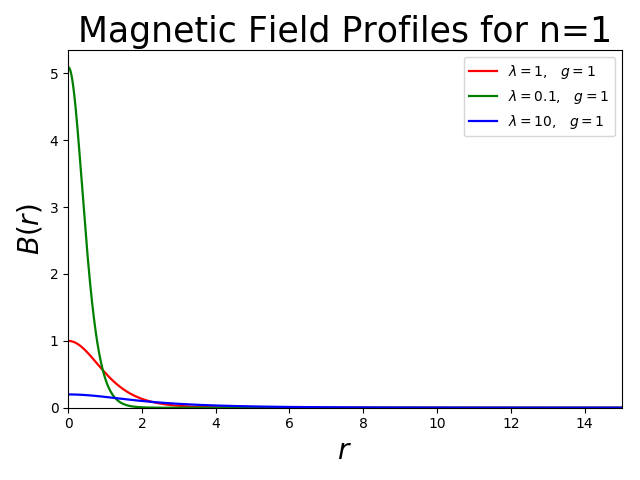
\includegraphics[scale=0.1]{Background_Folder/figures/solution_n1_magnetic_field_g_lambda.png}
        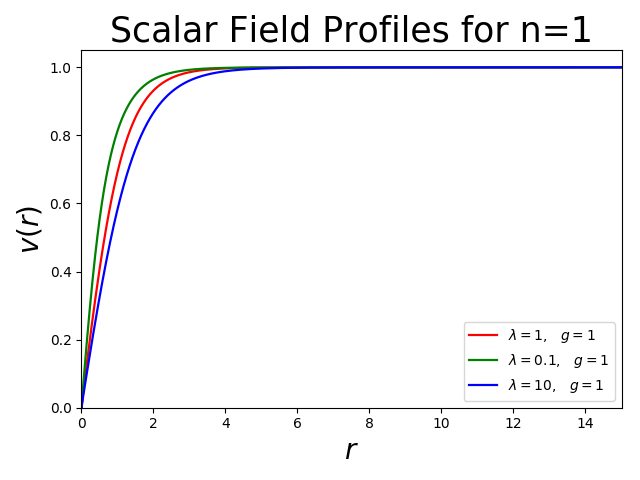
\includegraphics[scale=0.1]{Background_Folder/figures/solution_n1_scalar_field_g_lambda.png}
	\end{tabular}
    \caption[This figure depicts the magnetic and scalar field profiles in the \textcolor{red}{a}belian Higgs model.]{The profiles for the magnetic (left) and scalar (right) fields ($B(r)$ and $v(r)$, respectively) are depicted for winding number $n=1$, electromagnetic coupling $g=1$ and quartic interaction coupling $\lambda = (10,1,0.1)\times \lambda_c$. Here, $\lambda_c$ is the critical coupling, for which the BPS equations \eqref{eq:BPS1_Abel} hold.} \label{fig:Abelian_Higgs_Profiles_n1}
\end{figure}
    From the asymptotic equations \eqref{eq:Asymptotics1_Abelian_Higgs} and \eqref{eq:Asymptotics2_Abelian_Higgs}, we can recover the masses of the Higgs field and gauge field $m_{H}$ and $m_a$, respectively, in the Higgsed phase of the theory 
    \begin{align}
        m_{H}= \sqrt{2} m, \qquad m_a = \sqrt{2} \frac{g^2}{\lambda}m .
    \end{align}
    From the from of the propagator for scalar and vector theories, we know that scalar fields act attractively, whereas gauge fields act repulsively for like-charged configurations. This tells us that when $m_a>m_H$, the scalar field decays slower than the gauge field, so if we were to place two vortices on the plane, we will observe an attractive force between them. Likewise, if  $m_a<m_H$, we expect the vortices to repel each other. This line of thought hints at us that there is a critical value of the couplings, where vortices are free (non-interacting). Here we present a more precise argument for this. In order to do this, we will \textcolor{red}{use} \textit{Bogomol'nyi's identity}
    \begin{align}
        |D_1 \phi|^2 + |D_2 \phi|^2 = |D_1 \phi \pm D_2 \phi|^2 \pm B |\phi|^2. \label{eq:Bogomolnyi}
    \end{align}
    Further, we re-express the potential by completing the square
    \begin{align}
        U(\phi)&=\frac{\lambda}{2} \left( |\phi|^2 - v^2 \right)^2 - \frac{m^2 v^2}{2}. \label{eq:potential_square}
    \end{align}
    Here we can ignore the constant since the energy is defined up to a constant (albeit an infinite one). Utili\textcolor{red}{s}ing \eqref{eq:Bogomolnyi} and \eqref{eq:potential_square} we reach the following expression for the energy of this configuration
    \begin{align}
        E &= 2 \pi \int r dr \bigg(\frac{1}{2 g^2}B^2 \pm B(|\phi|^2 -v^2) + \frac{\lambda}{2} \left(|\phi|^2 -v^2 \right)^2 \\ \nonumber 
        &+ |D_1\phi \pm i D_2 \phi|^2 \pm B v^2 \bigg) \\ \nonumber
        &= 2 \pi \int r dr \bigg[|D_1\phi \pm i D_2 \phi|^2 +\frac{1}{2}\left( \frac{B}{g} \pm \lambda \left(|\phi|^2 -v^2  \right) \right)^2   \\ \nonumber \\
        &\pm \left(1 - \frac{\sqrt{\lambda}}{g} \right) B \left(|\phi|^2 - v^2 \right) \bigg] \pm n v^2,
    \end{align}
    where we have used Stokes' theorem.
    \begin{align}
        \int r dr B = n.
    \end{align}
    In order to have no interaction between the vortices, we need the energy of the $n$ vortex, the bound state of n vortices, to be the same as the energy of $n$ separate vortices. This implies that there is no potential energy, hence no force between them. This condition is satisfied when
    \begin{align}
        |D_1\phi \pm i D_2 \phi|^2 =0&,  \qquad \frac{B}{g} \pm \lambda \left(|\phi|^2 -v^2  \right) =0, \label{eq:BPS1_Abel}\\
        \lambda &= g^2 .\label{eq:BPS2_Abel}
    \end{align}
    The above equations (\eqref{eq:BPS1_Abel} and \eqref{eq:BPS2_Abel}) are known as the \textit{BPS equations} of the vortex, named after the people who first discovered a non-interacting limit for solitonic solutions in field theory -- \textit{Bogomol'nyi, Prasad \& Sommerfield} \cite{Bogomolny:1975de} \cite{Prasad:1975kr}.
    

    \subsection{Particle-\textcolor{red}{v}ortex \textcolor{red}{d}uality}
    The considerations of the previous section are more general and they apply for more than just systems in $2+1d$\textcolor{red}{,} even though the details differ. In a general QFT, we have roughly two different types of quantum excitations. One is the familiar type of elementary excitations that appear through the standard procedure of canonical quantization, where we introduce creation and annihilation operators that insert particles at a given position. The other type is, as we have just seen from the previous section, of a \textit{solitonic nature} (such as vortices). In other words, a solution that we reach not through expanding around the free solution in a small coupling parameter, but is more generally associated with a stationary point parametrically far from the free theory. This makes these solutions grow in size and energy the smaller the coupling is\textcolor{red}{,} so studying them in the quantum regime becomes tricky. Luckily, because their masses become large at small coupling, they decouple from the theory so one can study the quantum theory of the elementary excitations on its own without worrying about the solitons. Unfortunately, going in the other direction in terms of coupling strength, the solitons become light and their importance grows but so do quantum corrections for the elementary excitations and we reach a regime, where we do not understand the theory. So how do we learn more about these strongly coupled theories? \\
    \indent One approach that has become ever more popular in the past few decades is the idea of a \textit{duality}. Duality suggests that instead of having one model or one Lagrangian that describes the physics of a system, we instead have two \textcolor{red}{\textit{dual theories}}. For example, a way in which duality can manifest itself is the following. Theory \textit{I} has elementary excitations that we can study at weak coupling and non-perturbative excitations which are inaccessible due their large mass. Whereas theory \textit{II} describes the solitons of theory \textit{I} as its own elementary excitations at weak coupling (and a small mass) and the solitons present in theory \textit{II} are in fact the elementary states of theory \textit{I}. If the non-perturbative states in these systems are vortices in $2+1$ dimensions, then we have a type of \textcolor{red}{s}trong-\textcolor{red}{w}eak duality called a \textit{Particle-Vortex (PV) duality}. \\
    \indent \textcolor{red}{PV duality was first studied by \textit{Peskin} \cite{Peskin:1977kp} in 1977 and, a few years later, by \textit{Dasgupta \& Halperin} \cite{Dasgupta:1981zz}.}\\
    \indent Since we now have a reasonable grasp of what vortices are, we are ready to introduce particle-vortex duality. And what better place to start than the \textcolor{red}{a}belian Higgs model from the last section \eqref{eq:Abelian_Higgs_Model}. Earlier\textcolor{red}{,} we saw that non-perturbative solutions exist in this theory. It turns out that a model exists where the vortices of the \textcolor{red}{a}belian Higgs model appear as elementary excitations. In other words, there is a duality between these two models
    \begin{align}
        S_{\text{AH}} \longleftrightarrow S_{\text{XY}},
    \end{align}
    where
    \begin{align}
        S_{\text{XY}} &= \int d^3x \, |\partial_{\mu}\tilde{\phi}|^2-m^2 |\tilde{\phi}|^2 - \frac{\tilde{\lambda}}{2} |\tilde{\phi}|^4.
    \end{align}
    $S_{\text{XY}}$ is the action for the so called \textit{XY model} and $S_{\text{AH}}$ is defined as in \eqref{eq:Abelian_Higgs_Model}. The matching of the physics in the different phases is summari\textcolor{red}{s}ed in table \eqref{table:PV_Duality}.
    \begin{table}
\begin{center}
  \begin{tabular}{| l | c | c | c|}
      \hline
    $m^2$           &  $>0$                  & $=0$                           &  $<0$                                               \\\hline
                    &  SB phase              & Wilson-Fisher &  Coulomb phase                                      \\                             
    $S_{\text{XY}}$ &  local ANO             &  fixed point                   &  $2d$ logarithmic                                   \\                           
                    &  vortices              &                                &  potential                                          \\\hline
                    &   Massive excitations  & Wilson-Fisher &  SB phase                                           \\                
    $S_{\text{AH}}$ &  in                    & fixed point                    &  global vortices                                    \\                                  
                    &  Coulomb phase         &                                &  $E\xrightarrow{V \rightarrow \infty} \infty$       \\                      
    \hline
  \end{tabular}
\end{center}
        \caption[This table shows the matching of the phases of the XY model and the \textcolor{red}{a}belian Higgs model.]{This table shows the matching of the phases of the XY model and the \textcolor{red}{a}belian Higgs model. The $m$ parameter corresponds to the mass in the XY model. Deforming the XY model with a positive mass squared is matched by a negative mass squared deformation on the side of the \textcolor{red}{a}belian Higgs model. At $m^2=0$, both models are at a critical point known as the Wilson Fisher fixed point. }
        \label{table:PV_Duality}
    \end{table}
In \cite{Karch:2016sxi}, the authors showed a link between this particle-vortex duality and bosonization. This naturally leads us to the next section, which focuses on Fermi-Bose duality.
%\textcolor{red}{***More to add***}\\
%-- Say something about the relation between particle-vortex duality and bosonization \cite{Karch:2016sxi, Murugan:2016zal} \\
%Some history, Abrikosov \cite{Abrikosov1957}, type $I$ and $II$ superconductors. Vortices are solitons -- this means that they are non-perturbative solutions to the equations of motion that are localized and stable.\\
%            - Topological vs Non-Topological\\
%            - Review other vortices such as Abrikosov, Abelian Higgs, Pure Chern-Simons, Non-abelian vortices
%

%    \begin{itemize}
%        \item Tong TASI Solitons \cite{hep-th/0509216}
%        \item Importance of BPS \cite{Bogomolny:1975de, Prasad1975}
%    \end{itemize}
        \section{Fermi-Bose Duality} \label{Fermi-Bose_sec}
        We already met the idea of duality in the previous section. In general, they tend to be an equivalence of two theories. Two different ways in which we can state the same physics. Some of them are functional integral analogs of the Fourier transform (for functionals) -- one phenomenon can be described either in coordinate or momentum space, by one action or another. This can be achieved by introducing a Lagrange multiplier field and integrating out the original fields \textcolor{red}{\cite{Barci:1995iy, Burgess:1993np}}. Others tend to arise in consequence of the idea of universality. Two models that flow to the same CFT in the IR will tend to be equivalent sufficiently close to the fixed point \textcolor{red}{\cite{Seiberg:1994bz, Seiberg:1994rs}}.
        Yet other types of duality are inspired by the study of black hole thermodynamics and the holographic principle, such as the AdS/CFT duality \textcolor{red}{\cite{Maldacena:1997re}}. Others still, seem to be a consequence of deep mathematical ideas, such as the level-rank duality \textcolor{red}{\cite{Nakanishi:1990hj, Mlawer:1990uv, Naculich:2007nc, Naculich:1990pa, Camperi:1990dk}}.\\
        \indent Whatever the fundamental reasons for their existence is, dualities are interesting beca\textcolor{red}{u}se they give us another point of view that allows us to explore and understand the world of fundamental physics in more depth. As Feynman once said, ``Every theoretical physicist who is any good knows six or seven different theoretical representations for exactly the same physics'' \cite{Feynman_quote}. And in the spirit of his words, here duality is one more representation we wish to understand.\\
        \indent As pointed out above, dualities come in many flavours and the models we are considering here play a role in more than one type. $O(N)/U(N)$ (scalar or fermion) models are holographically dual to higher spin gravitational theories \cite{Klebanov:2002ja}. This duality seems to persist even after deforming the theories with a Chern-Simons term in the large $N$ limit\cite{Aharony:2011jz}. Fermions in 2+1d can be shown to be dual to vector fields via a Fourier transform-like functional integral transformation that we described above \cite{Burgess:1993np, Barci:1995iy}. And pure Chern-Simons theories are level-rank dual to each other \cite{Naculich:1990pa, Camperi:1990dk, Mlawer:1990uv, Nakanishi:1990hj, Naculich:2007nc}. In this section, we will concentrate on a duality that has all of the above ingredients in some form ($SU(N)/U(N)$ scalars/fermions and CS vector fields) that combine into what's believed to be an IR duality. More precisely, we are talking about a set of dualities between $2+1d$ gauge theories that are collectively known as \textit{Fermi-Bose duality}.\\
        \indent The duality between fermions and bosons was first conjectured  in the supersymmetric context \cite{Giveon:2008zn, Benini:2011mf, Aharony:2013dha, Aharony:2014uya}. Evidence for the non-supersymmetric version of these dualities comes from large $N$ computations on both sides both at finite temperature \cite{Aharony:2012ns}  and at $T=0$ \cite{Giombi:2011kc}. Furthermore, there is compelling evidence that the duality holds at finite $N$ from supersymmetric theories flowing to their non-SUSY versions \cite{Jain:2013gza, Gur-Ari:2015pca}.\\
        \indent Since $U(N) = (SU(N)\times U(1))/\mathbb{Z}_N$, we can in principle have different Chern-Simons levels for the $SU(N)$ and $U(1)$ symmetries. We will denote a $U(N)$ Chern-Simons theory with levels $k_1$ and $k_2$ corresponding to the $SU(N)$ and $U(1)$ symmetries, respectively, as a $U(N)_{k_1,k_2}$ theory. Prior to the inclusion of matter in our model, we state an important fact about these theories. Namely, that some choices of gauge groups and levels are dual to others. This is known as \textit{level-rank duality}. It's generalization to include matter is the duality that we present below.\\
\indent \textcolor{red}{Before we proceed with the statement of the dualities, we shall need to make a brief statement about regularization schemes. In the study of QFTs, couplings generally get renormali\textcolor{red}{s}ed and Chern-Simons theory is no exception. Different regularization procedures make different aspects clearer or make different calculations simpler. The Fermi-Bose dualities are usually discussed in so-called \textit{Yang-Mills regularization}. This procedure is performed by integrating out the YM dynamics, which leave a quanti\textcolor{red}{s}ed level in the infrared. For more details into this calculation, the reader may consult \textit{Pisarski \& Rao} \cite{PhysRevD.32.2081}}\\
        \indent In \textcolor{red}{this} regularization\textcolor{red}{,} the Fermi-Bose dualities are as follows \cite{Aharony:2015mjs} 
            \begin{align}
                SU(N)_k + scalars &\longleftrightarrow \ \ U(k)_{-N +\frac{N_f}{2}, -N + \frac{N_f}{2}} \quad + fermions, \label{eq:Fermi-Bose_1} \\
                U(N)_{k,k} + scalars &\longleftrightarrow SU(k)_{-N +\frac{N_f}{2}}\qquad \ \ \ \quad+ fermions,  \label{eq:Fermi-Bose_2}\\
                U(N)_{k,k+N} + scalars &\longleftrightarrow \ \ U(k)_{-N +\frac{N_f}{2}, -N + \frac{N_f}{2}-k} \ + fermions.  \label{eq:Fermi-Bose_3}
            \end{align}
            The scalars on the LHS of these equations are assumed to be tuned to a critical interacting point of the RG flow, known as the \textit{Wilson-Fisher \textcolor{red}{(WF)} fixed point} \cite{Wilson:1971dc}. \textcolor{red}{The WF fixed point occurs in $\phi^4$ theory in dimensions $d<4$.} Similarly to \textcolor{red}{Particle-Vortex} duality, which maps elementary excitations to non-perturbative vortices, Fermi-Bose duality maps the fundamental perturbative states on one side to monopole \textcolor{red}{(Define monopole operators - Studied in theories without CS \cite{Borokhov:2002ib, Borokhov:2002cg, Pufu:2013eda, Pufu:2013vpa})}  or baryon operators on the other side. \textcolor{red}{A monopole operator $\mathcal{M}(x)$ is defined as inserting a unit of flux at a point $x$. This means that in the path integral we integrate over configurations with a fixed flux emanating from the point $x$} \\
\begin{align}
    \textcolor{red}{ \langle \mathcal{M}(x) \rangle = \int \mathcal{D}A_{\mu} e^{i S}\bigg |_{\frac{1}{4\pi} \int_{\textbf{S}^2} d^2S_{\mu} \epsilon^{\mu \nu \rho}F_{\nu \rho} =1}, }
\end{align}
    \textcolor{red}{where $\mathbf{S}^2$ is a sphere surrounding the monopole insertion point.} \\
            \indent Understanding the details of this duality subject to the inclusion of a chemical potential has been the formative motivation for this work. We believe that some of the results of this thesis have sown the seed for this understanding. More specifically, the role of the ground state discussed in chapter 3 in the duality still remains mysterious. The resolution of this mystery is left for future work. Thus we conclude our discussion of Fermi-Bose duality and move on to the physics of non-commutative fluids\textcolor{red}{.}
%\textcolor{red}{***More to add***}\\
%            - Make sure to include the first bosonization papers \cite{hep-th/9407078, hep-th/9407182} \\
%            - Explain what is the precise dictionary of this duality. The two theories are equivalent but which degrees of freedom correspond to which. Clarify that fundamental perturbative states on one side map to monopole operators on the other and vice-versa.\\
%            - Monopole operators
%
        \section{Non-Commutative Fluids}
    In this section we will define important physical notions in a \textit{non-commutative geometry}, show how it relates to the theory of fluids and demonstrate how the non-commutative version of the Landau problem leads directly to the non-commutative Chern-Simons action. Finally, we discuss the Fock space of this action to prepare the presentation of results that we have discovered. For a good summary of this topic, we refer the reader to this set of excellent reviews on physics on non-commutative geometry \cite{Polychronakos:2007df, Szabo:2001kg, Douglas:2001ba}.

    Non-commutative geometry can arise naturally from the quantization of a particle's phase space coordinates. The simplest way to see this connection is through the Heisenberg algebra of the canonical commutation relations
    \begin{align}
        [\hat{x}, \hat{p}] = i \hbar.
    \end{align}
    As is well known, this quantization condition leads to a ``smearing out`` of the phase space structure of the theory. It makes it so that the notion of a point in phase space no longer makes sense, since one can no longer measure both position and momentum accurately. \\
    \indent However, there are more exotic cases, where the coordinate space becomes non-commutative or fuzzy, due to the specific form of the Poisson brackets in the problem. In such a problem, the notion of a point in space is no longer reasonable and one can no longer measure the position of a (quasi)particle to arbitrary accuracy on both axes at once. An example of a problem, where the different momenta exhibit such non-commutativity is the problem of particles in a magnetic field that we discussed earlier. Similarly, we all know that angular momentum also behaves in a non-commutative way so the idea of the spatial coordinates having non-zero commutator comes naturally. Finally, in the study of fluids, one can define a type of Poisson bracket that is restricted to the coordinate space, which leads to a non-commutative space following a canonical quantization \cite{Jackiw:2002pn}. These ideas of a non-commuting space-time were first explored by \textit{Snyder} in 1947 \cite{Snyder:1946qz, Snyder:1947nq}.
    \subsection{Review of \textcolor{red}{n}on-\textcolor{red}{c}ommutative \textcolor{red}{g}eometry}
    Let us see how to define a \textit{non-commutative space}. Here we will be concerned with a $D$ dimensional space-time that has both a set of $D-2p$ commuting $\{ y_i, \ i=2p+1,...,D\}$ and $2p$ non-commuting coordinates $\{ x_i, \ \alpha =1,...,2p\}$. More precisely,
    \begin{align}
        [y_i, y_j] &=0,\\
        [x_{\alpha}, x_{\beta}] &=i \bm{\theta}_{\alpha \beta}, \label{eq:space_time_commutations}
    \end{align}
    where $\theta$ is an anti-symmetric constant one-form. One can perform linear transformations on the coordinates $x_{\alpha}$ so that the matrix $\theta$ is in canonical block form
    \begin{align}
        \bm{\theta}_{\alpha \beta } = \theta \begin{bmatrix}
            i \bm{\sigma_2} &  & \text{\huge0} \\
                     & \ddots &  \\
                    \text{\huge0} &  & i \bm{\sigma_2} \\
                \end{bmatrix},
    \end{align}
    where 
    \begin{align}
        i \bm{\sigma_2} = \begin{bmatrix}
            0 & 1 \\
            -1 & 0 \\
        \end{bmatrix}.
    \end{align}
    This leaves us with $p$ pairs of the Heisenberg algebra
    \begin{align}
        [x_{2\alpha -1}, x_{2\alpha}]=i\theta, \qquad \alpha=1,...,p.
    \end{align}
    This quantization of the spatial coordinates leads to the existence of a Hilbert space. Since we can now think of the coordinates as operators, then each operator has a set of eigenstates with associated quantum numbers. To make this more explicit, let us define the \textit{creation}, \textit{annihilation} and \textit{number} operators
    \begin{align}
        \bm{a}_{\alpha} = \frac{x_{2\alpha-1} +i x_{2\alpha}}{\sqrt{2 \theta}}, \qquad \bm{a}^{\dag}_{\alpha} &= \frac{x_{2\alpha-1} -i x_{2\alpha}}{\sqrt{2 \theta}}, \\
        \bm{n}_{\alpha} = \bm{a}^{\dag}_{\alpha}\bm{a}_{\alpha}.
    \end{align}
    These operators allow us to build the familiar \textit{Fock space} from QFT by acting on a vacuum state
    \begin{align}
        |n_1,...,n_p\rangle=  \bm{a}^{\dag}_1^{n_1}... \bm{a}^{\dag}_p^{n_p}|0\rangle.
    \end{align}

    Further, we define the derivative operators through the relations
    \begin{align}
        \partial_{\mu} \cdot x_{\nu} = [\partial_{\mu}, x_{\nu}] = \delta_{\mu \nu}, \qquad \mu,\nu = 1,...,D.
    \end{align}
    Specifically for the non-commuting coordinates
    \begin{align}
        \partial_{\alpha}= -i \omega_{\alpha \beta} x_{\beta}, \qquad \alpha, \beta = 1,...,2p,
    \end{align}
    where $\omega_{\alpha \beta} = \left(\theta^{-1} \right)_{\alpha \beta}$. From here it follows that
    \begin{align}
        [\partial_{\alpha}, \partial_{\beta}] = i \omega_{\alpha \beta}.
    \end{align}


    \subsection{Non-\textcolor{red}{c}ommutative \textcolor{red}{f}ield \textcolor{red}{t}heory}

    Now that we understand some of the basic ideas of non-commutative geometry, we would like to define a field theory on this non-commutative space. The simplest possible gauge theory contains just a gauge field $A_{\mu}$. Further, the easiest way to construct a gauge invariant theory is by forming an action that is composed of a trace of covariant derivatives 
    \begin{align}
        D_{\mu} = -i \partial_{\mu} + A_{\mu},
    \end{align}
    since under a gauge transformation $D_{\mu}$ transforms as
    \begin{align}
        D_{\mu} \rightarrow U D_{\mu} U^{-1}.
    \end{align}
    Restricting ourselves to the non-commuting submanifold, we have
    \begin{align}
        D_{\alpha} &= -i \partial_{\alpha} + A_{\alpha} = \omega_{\alpha \beta}x^{\beta}+ A_{\alpha} = \omega_{\alpha \beta} \left( x^{\beta}+ \theta^{\beta \gamma} A_{\gamma} \right) \equiv \omega_{\alpha \beta} X^{\beta}.
    \end{align}
    

    \\ 
    - Specifically, non-commutative Chern-Simons theory arises as the action of a massless particle confined to the plane in the presence of a magnetic field. \cite{Polychronakos:2001mi} Let us take a look at the action of a particle of charge $q$ and mass $m$ moving in an electromagnetic field generated by the four-potential $A^{\mu} = \left(-V(\bm{x}, t), \ \bm{A}(\bm{x},t)\right)$
    \begin{align}
        S = \int dt \left(\frac{1}{2} m^2 v^2 - q V(\bm{x},t) + q \bm{v} \cdot \bm{A}(\bm{x},t)\right). \label{eq:Lagrangian_Charged_Particle_In_EM_Field}
    \end{align}
    Now, let us assume that the particle is massless and in addition, it is in a constant magnetic field and the electric potential is 0. Since $\nabla \times \bm{A} = \bm{B}$, this implies that
    \begin{align}
        A_i = \frac{B}{2} \epsilon_{i j} x_j \label{eq:Gauge_Potential_Constant_B_Field},
    \end{align}
    where $B= |\bm{B}|$.
    Substituting Equation \eqref{eq:Gauge_Potential_Constant_B_Field}  into Equation \eqref{eq:Lagrangian_Charged_Particle_In_EM_Field}, we arrive at the action
    \begin{align}
        S = \int dt \left( q \frac{B}{2}\epsilon_{i j} \dot{x_i} x_j \right).
    \end{align}
    From here we proceed by making the identification
    \begin{align}
        x_i \leftrightarrow X_i.
    \end{align}
    And since the $X_i$'s transform under gauge transformations, we ought to make sure that the action remains invariant. To this end, we need to also gauge the time derivative $\partial_0 \rightarrow D_0 = \partial_0 +A_0$
    \begin{align}
        S = \int dt \ \left[ q \frac{B}{2} \epsilon_{ij} Tr \left(D_0 X^i X^j \right) \right] = \int dt \ \left[ q \frac{B}{2} \epsilon_{ij} Tr \left(\partial_0 X^i X^j + [A_0, X^i] X^j \right) \right].
    \end{align}
    The introduction of the time component of the gauge field leads to a Gauss's law constraint
    \begin{align}
        [X^1, X^2] =0.
    \end{align}
    It seems that this constraint has removed the non-commutativity that we tried to introduce into our model. In order to bring it back, we add an extra term to the action such that we get the Heisenberg algebra \eqref{eq:space_time_commutations} that we explored earlier
    \begin{align}
        S =\int dt \ \left[ q \frac{B}{2} \epsilon_{ij} Tr \left(\partial_0 X^i X^j + [A_0, X^i] X^j + 2 \theta A_0 \right) \right].
    \end{align}
    Thus we have arrived at the non-commutative abelian Chern-Simons model by considering the movement of charged particles in a magnetic field confined to a two-dimensional plane.

    

